\documentclass[
	a4paper,     		%% Papiergroesse: A4 OBSOLETE
%	twoside,     		%% Zweiseitiges Layout (alternativ: oneside)
	headsepline, 		%% Horizontale Linie unter Kopfzeile
	footsepline, 		%% Horizontale Linie ueber Fusszeile
	titlepage,   		%% Eigenstaendige Titelseite (alternativ: notitlepage)
%	halfparskip, 		%% Halbe Leerzeile zwischen zwei Abschnitten (alternativ: parskip, ...)
	12pt,        		%% Schriftgroesse: 12pt (alternativ: 10pt, 11pt, ...) OBSOLETE
%	bibtotoc,			%% Bilbiographie in's Inhaltsverzeichnis aufnehmen
%	liststotoc,			%% Indexe in's Inhaltsverzeichnis aufnehmen
%	smallheadings,		%% Kleine Ueberschriften
%	DIV1,				%% Divisor, Zeilenlänge ca. 70 Zeichen
%	BCOR01cm,			%% Bindekorrektur
% 	draft			  	%% Entwurfsmodus, volle/leere Boxen markieren
%	abstracton			%% Titel "`Zusammenfassung"' einschalten
]{scrreprt}

%%%
%%% Pakete
%%%

%%% Glossar
% \usepackage[german]{gloss}
% \newcommand{\acr}[1]{{\small\gloss[word]{#1}}}
% 
% \newcommand{\abk}[1]{#1\xdot}
% \DeclareRobustCommand\xdot{\futurelet\token\Xdot}
% \def\Xdot{\ifx\token\bgroup.\else\ifx\token\egroup.\else
%   \ifx\token\/.\else\ifx\token\ .\else\ifx\token!.\else
%   \ifx\token,.\else\ifx\token:.\else\ifx\token;.\else
%   \ifx\token?.\else\ifx\token/.\else\ifx\token'.\else
%   \ifx\token).\else\ifx\token-.\else\ifx\token+.\else
%   \ifx\token~.\else
%   \ifx\token.\else.\ \fi\fi\fi\fi\fi\fi\fi\fi\fi\fi\fi\fi\fi\fi\fi\fi} 
% \newcommand{\zB}{\mbox{z.\,B}\xdot}

%%% Literaturverzeichnis, deutschen Stil benutzen (dinat)
%%% TODO: funktioniert leider derzeit nicht mit TeXlipse!
%\usepackage[square]{natbib}
%\citestyle{dinat}

%%% Grafik
\usepackage{pstricks}

%%% Subfigures
\usepackage{subfig}

%%% UML
%\usepackage{pst-node}
%\usepackage{pst-uml}
%\let\umlClass\pstumlClass	%%% workaround: pst-uml und uml kollidieren
%\usepackage{uml}

%%% Deutsche Sprache verwenden
\usepackage{ngerman}

%%% Kodierung der Eingabezeichen setzen (fuer dt. Umlaute etc.)
%%% Für Linux: [latin1] für Windows: [ansinew]
\usepackage[utf8]{inputenc}

%%% Zeichen-Kodierung in PDF-Dokumenten
\usepackage[T1]{fontenc}
%\usepackage{ae,aecompl}

%%% Web-Addressen auch mit T1-Encoding
\usepackage[T1]{url}
%%% ... und in tt-Font
\urlstyle{tt}

%%% amsmath, amssymb, amstext: Unterstuetzung div. mathematischer Zeichen etc.
\usepackage{amsmath,amssymb,amstext}

%%% pifont: "pifont Xs and Check Marks"
% \usepackage{pifont}

%%% PostScript-Fonts ersetzen
\usepackage{psfrag}

%%% Programmcode einbinden, Listings
\usepackage{listings}

%%% Farb-Unterstuetzung
\usepackage{color}

%%% Tabellen
\usepackage{booktabs}
\usepackage{array}
\usepackage{multirow}
\usepackage{tabularx}
\usepackage{threeparttable}	% Fussnoten in table-Umgebung

%%% Floats strikter positionieren (Option 'H'ere)
\usepackage{float}

%%%
%%% Pakete konfigurieren, Definitionen
%%%

%%% Ueberschriften bis zur Ebene 3 nummerieren
\setcounter{secnumdepth}{3}

\setcounter{tocdepth}{3}

%%% Neue Spaltentypen definieren
\newcolumntype{N}{>{\bfseries\scriptsize}l}
\newcolumntype{V}[1]{
	>{\bfseries\scriptsize\raggedright\hspace{0pt}}p{#1}
}

%%% Ein paar Farbdefinitionen (s. http://texnik.de/listings/listing0.pdf)
% \definecolor{hellgelb}{rgb}{1,1,0.8}
% \definecolor{hellgrau}{rgb}{0.95,0.95,0.95}
% \definecolor{colKeys}{rgb}{0,0,1}
% \definecolor{colIdentifier}{rgb}{0,0,0}
% \definecolor{colComments}{rgb}{1,0,0}
% \definecolor{colString}{rgb}{0,0.5,0}

%%% Konfiguration des listing-Paketes
% \lstset{%
% 	float=hbp,%
% 	%basicstyle=\ttfamily\footnotesize, %
% 	identifierstyle=\color{colIdentifier}, %
% 	basicstyle=\small,%
% 	stringstyle=\ttfamily,%
% 	keywordstyle=\color{colKeys}, %
% 	stringstyle=\color{colString}, %
% 	commentstyle=\color{colComments}, %
% 	columns=flexible, %
% 	tabsize=2, %
% 	frame=tb, %
% 	extendedchars=true, %
% 	showspaces=false, %
% 	showstringspaces=false, % 
% 	numbers=left, %
% 	numberstyle=\tiny, %
% 	breaklines=true, %
% 	backgroundcolor=\color{hellgrau}, %
% 	breakautoindent=true, %
% 	captionpos=b%,
% 	aboveskip=\bigskipamount,%
% 	belowskip=\medskipamount,%
% 	escapeinside={(*}{*)}, %
% 	mathescape, %
% 	language=Pseudo, %
% }

%%% Benoetigte Sprachen laden
% \lstloadlanguages{Pseudo}

%%%
%%% Seitenlayout, Schriften
%%%

%%% scrpage2: KOMA Kopf- und Fusszeile
\usepackage[automark]{scrpage2}

%%% KOMA-Script: Optionen
% \KOMAoptions{fontsize=12pt}
% \KOMAoptions{paper=a4}

%%% EM unterstrichen darstellen
%\usepackage{ulem}

%%% Schrift fuer Captions verkleinern
\setkomafont{captionlabel}{\scriptsize}
\setkomafont{caption}{\usekomafont{captionlabel}}

%%% Schrift fuer Ueberschriften umstellen
%\setkomafont{sectioning}{\normalcolor\bfseries}

%%% Schriften fuer Titel- und Fusszeile umstellen
%\setkomafont{pagehead}{\normalfont\sffamily}
\setkomafont{pagenumber}{\normalfont\rmfamily\slshape}

%%%
%%% PDF-Einstellungen
%%%

%%% Fallunterscheidung: PDF- oder 'normale' Erstellung?
\usepackage{ifpdf}

%%% Falls wir PDF erzeugen...
\ifpdf
  %%% Serifenlose Schriften benutzen
  \usepackage{mathpazo}
  \usepackage[scaled=.95]{helvet}
  \usepackage{courier}	
  \renewcommand{\familydefault}{\sfdefault}
  \usepackage[sf]{titlesec}

  %%% Unterstuetzung fuer Grafiken
  \usepackage[pdftex]{graphicx}
 
  %%% Kompressionslevel: 0-9
  \pdfcompresslevel=9

	%%% Informationen ueber das PDF-Dokument setzen
	\hypersetup{
	  pdftitle={Peer-to-Peer-Netzwerke: Pastry und Tapestry},%
	  pdfauthor={Christian Kungel (christian.kungel@htwg-konstanz.de),%
				 Daniel Seidel (daniel.seidel@htwg-konstanz.de),%
	  			 Jan Tammen (jan.tammen@htwg-konstanz.de)},%
	  pdfsubject={Verteilte Systeme 2},%
	  pdfcreator={Jan Tammen (jan.tammen@htwg-konstanz.de)},%
	  pdfkeywords={P2P, Peer-to-peer, Pastry, Tapestry},
	  pdfproducer={\LaTeX\ with package \flqq hyperref\frqq}, %%
	  bookmarksopen=true,
	  pdfpagemode=UseOutlines,
	  pdfview=FitV, % FitH
	  pdfstartview=FitV,
	  pdfhighlight=/I,
	%   pdfborder=0 0 0, % keine Box um die Links!
	  bookmarksnumbered=false,
	  plainpages=false,
	}

	%%% Dateiendung fuer Grafiken setzen -- so kann beim Einbinden der Grafik
	%%% auf die Endung verzichtet werden und es wird automatisch die korrekte 
	%%% Datei ausgewaehlt (.eps / .pdf)
  \DeclareGraphicsExtensions{.pdf}
  
  %%% Pfad fuer Bilder setzen
  \graphicspath{{../images}}

%%% ... oder im 'normalen' Modus sind
\else

  %%% Unterstuetzung fuer Grafiken
  \usepackage[dvips]{graphicx}

  %%% s.o.
  \DeclareGraphicsExtensions{.eps}
  \graphicspath{{../images}}

  %%% Hyperlinks in PS-Dokumenten, Optionen s.o.
  \usepackage[%
    dvips,
    colorlinks=false,
    breaklinks=true,				%% Duerfen Links umbrochen werden? (true|false)
  ]{hyperref}

\fi

%%% Links im dvips-Mode auch umbrechen
\usepackage{breakurl}

%%%
%%% Layout der Titelseite
%%%

%%% Titelkopf, erscheint oberhalb des Titels
\titlehead{
	\begin{figure}[H]
		\centering
		
\includegraphics[width=\textwidth]{../images/htwg-logo}
	\end{figure}
}

%%%% Subject, erscheint oberhalb des Titels
\subject{Seminar Verteilte Systeme II, SS 07}

%%% Titel
\title{Pastry und Tapestry}


%%% Publisher, hier: Verantwortlicher Prof.
\publishers{%
	\small
  Prof.\ Dr.-Ing.\,Wäsch, Fakultät Informatik, HTWG Konstanz
}

%%%% Autor. Weitere Autoren mit \and{<Name>} hinzufuegen
\author{%
	Christian Kungel
	\and{%
		Daniel Seidel
	}%
	\and{%
		Jan Tammen
	}%
}%

%%% Datum setzen
\date{\today}

%%% Rueckseite der Titelseite
\lowertitleback{%
	\footnotesize%
	Erstellt mit \LaTeXe\ unter Verwendung des \KOMAScript-Pakets.
}

%%%
%%% Header und Footer
%%%

\pagestyle{scrheadings}

%%% Kopfzeile in den Rand ragen lassen
%\setheadwidth{textwithmarginpar}

%%% Fusszeile in den Rand ragen lassen
%\setfootwidth{head}

%%% \automark[rechte Seite]{linke Seite}
%\automark[subsection]{section}

%% Header links -- section
%\ihead[]{\rightmark}

%% Header rechts -- chapter
%\ohead[]{\leftmark}

%% Header mittig -- leer
\chead[]{}

%% Footer mittig -- leer
\cfoot[]{}

%% Footer rechts -- Seitenzahl
\ofoot[]{\thepage}

%%% Footer links -- Titel der Arbeit
\ifoot[]{\footnotesize{Pastry und Tapestry}}

%%%
%%% Sonstiges
%%%

%%% Glossar und Index erstellen 
% \makegloss
% \makeindex

%%%
%%% Beginn Hauptdokument
%%%
\begin{document}

%%% Titelseite erstellen
\maketitle

%%% Ehrenwörtliche Erklärung
\thispagestyle{empty}
\section*{Ehrenw\"{o}rtliche Erkl\"{a}rung}
\addcontentsline{toc}{section}{Ehrenwörtliche Erklärung}

Hiermit erklären wir, Daniel Seidel (276446), Christian Kungel (279475) und Jan Tammen 
(277143),

\vspace{1.0 cm}
\begin{enumerate}
  \item dass wir die Ausarbeitung mit dem Titel:\\
  
  \textbf{"`Pastry und Tapestry"'}\\
  
  selbständig und ohne fremde Hilfe angefertigt haben und keine anderen als im
  Quellenverzeichnis genannten Hilfen benutzt haben;
  
  \item dass wir die Übernahme wörtlicher Zitate, Tabellen, Zeichnungen, Bilder
  und Programme aus der Literatur oder anderen Quellen (Internet) sowie die
  Verwendung der Gedanken anderer Autoren an den entsprechenden Stellen innerhalb
  der Arbeit gekennzeichnet haben.
\end{enumerate}

\vspace{1.0 cm}
Wir sind uns bewusst, dass eine falsche Erklärung als Täuschungsversuch
gewertet wird.

\vfill Konstanz, \today

%%% Inhaltsverzeichnis erstellen
%\newpage
\tableofcontents

%%% Bildverzeichnis erstellen
\newpage
\listoffigures

%%% Tabellenverzeichnis erstellen
%\newpage
%\listoftables

%%%
%%% Beginn Inhalt
%%%
\chapter{Einleitung Peer-to-Peer-Netzwerke}
\section{The Mozart Programming System}
In der vorliegenden Ausarbeitung soll das "`Mozart Programming System"'
\footnote{\url{http://www.mozart-oz.org}} 
vorgestellt werden. Bei \textsl{Mozart} handelt es sich um eine 
Programmierumgebung, die die multiparadigmische Programmiersprache \textsl{Oz} 
implementiert.

Entstanden ist Mozart-Oz ursprünglich als Forschungsprojekt am Deutschen 
Forschungszentrum für Künstliche Intelligenz (DFKI) sowie der Universität 
Saarbrücken. Inzwischen wird die Sprache vom Mozart-Konsortium, zu welchem 
Arbeitsgruppen aus Belgien, Schweden und Deutschland gehören, weiterentwickelt. 
Die Quellen sind unter einer Open-Source-Lizenz verfügbar; ein kommerzieller 
Einsatz der Sprache ist ebenfalls möglich.

Ähnlich wie in Java können Oz-Programme in eine Art Byte-Code übersetzt werden 
und laufen anschließend in einer virtuellen Maschine ab. Auf diese Weise wird 
eine gewisse Plattformunabhängigkeit erreicht.

\section{Die Programmiersprache Oz}
\subsection{Features}
Als Hauptfeatures und -vorteile von Oz gelten die folgenden Aspekte:

\begin{description}
  \item[Nebenläufigkeit] Arbeit mit leichtgewichtigen Threads, 
  Datenfluss-Synchronisation.
  \item[Inferencing] Constraintbasierte und 
  logische Programmierung.
  \item[Verteilung] Transparente 
  Netzwerkunterstützung.
  \item[Flexibilität] Dynamische Typisierung, inkrementelles 
  Kompilieren.
\end{description}

\subsection{Datentypen}
Die Sprache stellt eine Reihe von Datentypen zur Verfügung, deren Hierarchie in 
Abbildung \ref{fig:oz-datentypen} dargestellt ist.

\begin{figure}[hp]
  \centering 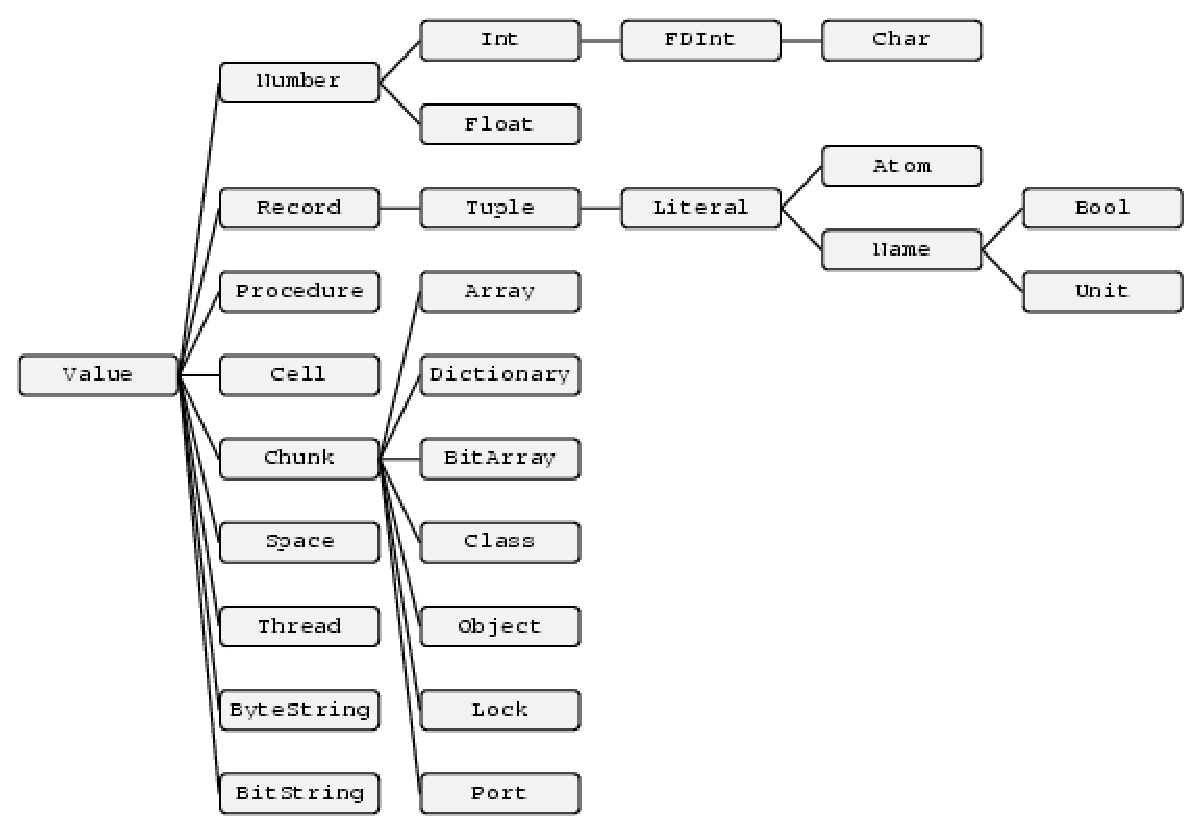
\includegraphics[width=0.70\textwidth]{../images/oz-datentypen} 
  \caption{Hierarchie der Datentypen in Oz 3. Quelle:
  \cite[Tutorial of Oz, Chapter 3.1]{url:mozart-documentation}}
  \label{fig:oz-datentypen}
\end{figure}

Einige der wichtigsten Datentypen seien hier kurz aufgeführt (vgl. 
\cite{Brunklaus:00}).

\begin{enumerate}
  \item Einfache Werte
    \begin{description}
      \item [Zahlen] können in Oz sowohl als ganze Zahlen (\texttt{Int, Char})
      als auch Fließkommazahlen (\texttt{Float}) benutzt werden.
      \item[Literale] teilen sich auf in sog. Atome und Namen. Ein Atom wird 
      durch eine alphanumerische Zeichenkette beschrieben, die entweder mit 
      einem Kleinbuchstaben beginnt oder in Hochkomma gefasst ist. Namen sind 
      eindeutige Bezeichner, die über eine spezielle Prozedur namens 
      \texttt{NewName} erzeugt werden können.
      \item[Prozeduren] können in Oz an Variablen gebunden und auch zur 
      Laufzeit erzeugt werden. \end{description}
  \item Zusammengesetzte Werte
    \begin{description}
      \item[Records] bestehen aus einem Bezeichner (Label) sowie einer festen 
      Anzahl von Komponenten oder Argumenten. Argumente bestehen aus dem Tupel 
      (Feature, Feld).
      \item[Tupel] sind ein Spezialfall von Records, bei denen die Argumente 
      kein explizites Feature besitzen.
      \item[Listen] sind eine Sonderform der Tupel. Die leere Liste wird mit
      \texttt{nil} denotiert, offene Listen bspw. als \texttt{1|2|3|nil} und 
      geschlossene Listen (also Listen mit fester Elementanzahl) als \texttt{[1 
      2 3]}.
    \end{description}
  \item \textbf{Chunks} erlauben es, abstrakte Datentypen zu konstruieren. 
  Oz bringt bereits einige vordefinierte Chunks mit, z.B. \texttt{Array} 
  oder \texttt{Dictionary}.
\end{enumerate}

\subsection{Multiparadigmisch?}
Wie bereits eingangs erwähnt, unterstützt Oz mehrere Programmierparadigmen:

\begin{enumerate}
  \item Constraint-Programmierung
  \item Funktionale Programmierung
  \item Objektorientierte Programmierung
  \item Logische Programmierung
\end{enumerate}
  
Im Gegensatz zu einer Programmiersprache, die nur eines der Paradigmen 
unterstützt, lassen sich in Oz also die zu lösenden Probleme von mehreren 
Seiten gleichzeitig mit dem jeweils geeignetsten Paradigma bearbeiten. 
Erreichen könnte man dies zwar auch durch die Kombination verschiedener 
Programmiersprachen, dabei bliebe aber der Nachteil, dass man semantische 
Lücken überwinden und Schnittstellen zwischen den einzelnen Sprachen definieren 
müsste. Dies würde u.a. zu einer aufwendigeren Fehlersuche führen. Mit Oz 
lassen sich hingegen die verschiedene Paradigmen problemlos miteinander 
kombinieren, deren gemeinsame Basis, das Oz Programming Model, im nächsten 
Abschnitt vorgestellt wird.

\subsection{Programmiermodell (Oz Programming Model, OPM)}
Die Grundlage für Berechnungen in Oz bildet das so genannte \textsl{Concurrent 
Constraint Programming}. Alle weiteren Paradigmen werden durch sog. "`syntactic 
sugar"' (Syntaxerweiterungen) in die Sprache integriert \cite{KI-LP96}.

Allgemein verwendet das Modell für Berechnungen die Metapher eines sog. 
\textsl{Berechnungsraums} (Computational Space). In diesem befindet sich zum 
einen ein \textsl{Speicher}, zum anderen eine Anzahl von sog. \textsl{Aktoren}. 
Aktoren führen die eigentlich Berechnung durch, indem sie schrittweise 
reduziert werden und sich dabei über den gemeinsamen Speicher synchronisieren. 
Dazu können Aktoren Information in den Speicher schreiben (tell) und auf 
Information warten und diese anfordern (ask).

Nebenläufigkeit (Concurrency) ist einer der wichtigsten Aspekte des OPM. Dabei 
bedeutet Nebenläufigkeit, dass verschiedene Berechnungen unabhängig voneinander 
durchgeführt werden können, nicht, dass diese parallel ablaufen.


\chapter{Pastry}
\begin{quote}
"`\textbf{Pastry} is a generic, scalable and efficient substrate for peer-to-peer 
applications. Pastry nodes form a decentralized, self-organizing and 
fault-tolerant overlay network within the Internet. Pastry provides efficient 
request routing, deterministic object location, and load balancing in an 
application-independent manner. Furthermore, Pastry provides mechanisms that 
support and facilitate application-specific object replication, caching, and 
fault recovery."'
\end{quote}

\section{Grundlagen}
Jeder Knoten erhält eine eindeutige 128 bit Adresse (NodeID).
Dies geschieht entweder zufällig, oder durch eine Verschlüsselungsfunktion, die
auf die IP Adresse angewendet wird. Die NodeID's bilden also einen Ring von
$0-2^{128}$ (vgl. \cite{Schindelhauer2004}).

\section{Struktur}
\label{struktur}
Pastry verwaltet drei unterschiedliche Informations-Mengen. Das
sind: 
\begin{itemize}
  \item Routing Tabelle
  \item Leaf Set
  \item Neighbourhood Set
\end{itemize}
In der Routing Tabelle sind Einträge der Art NodeID $\rightarrow$ (IP)Adresse
vorhanden. 
\begin{quote}
''Jeder Peer kennt für jeden Präfix $p$ der NodeID über dem Alphabet
$2^b$ und für jeden Buchstaben $x \epsilon \{0, . . . , 2^{b - 1}\}$ einen
Repräsentanten der mit $px$ anfängt''\cite{Schindelhauer2004}. 
\end{quote}  
Ist beispielsweise $b=2$ und $2^b=4$, werden also $2^{2}-1 = 3$ Einträge für
jeden Präfix des Knotens gespeichert (siehe Abb. \ref{pastryPointer}).
\newline Das Leaf
Set enthält NodeIDs numerisch naheliegender Knoten, also
den benachbarten Knoten gemäß der Anordnung auf dem Ring. Ist $l$ die Größe des
Leaf Sets, werden $l/2$ linke Nachbarn und $l/2$ rechte Nachbarn gespeichert
\cite{Schindelhauer2004}(siehe Abb. \ref{pastryPointer}). Beim
Einfügen neuer Knoten wird das Leaf Set stets aktualisiert. 

\begin{figure}[H]
  \centering 
  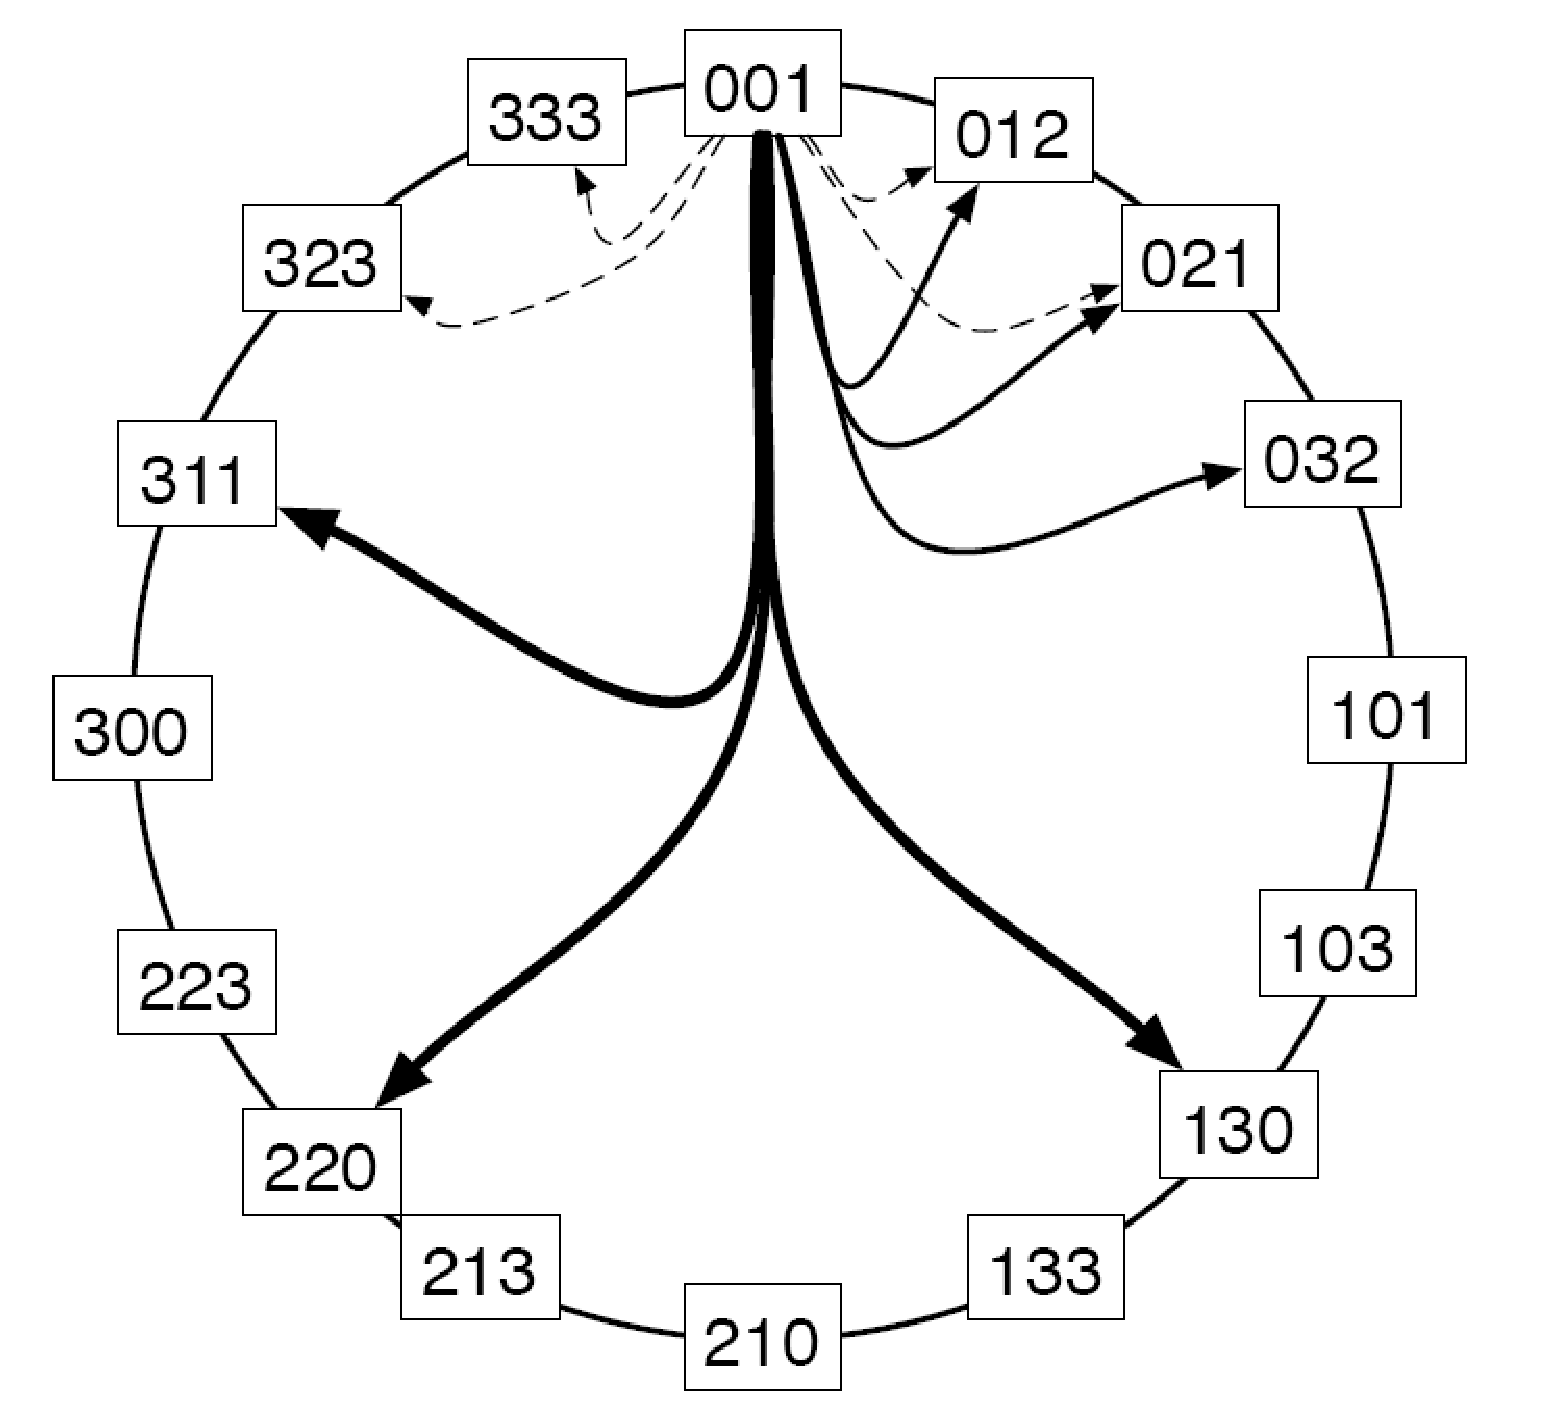
\includegraphics[width=0.5\textwidth]{../images/pastryPointer}
  \caption[Pastry Pointer]{Leaf Set(gestrichelt) und Routing Tabelle
  (durchgezogen) des Knotens $001$ für $b=2$ und $l=4$ \cite{Schindelhauer2004}}
  \label{pastryPointer}
\end{figure}
Im Neighbourhood Set werden Knoten gehalten, die
netzwerk-topologisch naheliegen. Dies wird durch heuristische Ansätze wie
PING-Zeit etc. realisiert.

\section{Routing}
Sollen nun Datenpakete weitergeleitet (geroutet) werden, macht man sich die im
vorangegangen Kapitel \ref{struktur} eingeführten Informationsmengen wie folgt
zunutze: 
\begin{enumerate}
  \item Durchsuche das Leaf Set nach dem Zielknoten. Ist er enthalten, wird das
  Paket dorthin weitergeleitet.
  \item Ansonsten wird die übereinstimmende Präfixlänge bestimmt, um das Paket
  anschließend an einen Knoten zu senden, dessen Präfix mindestens in einer
  Stelle mehr mit dem Zielknoten übereinstimmt.
  \item Schlägt dies ebenfalls fehl, werden alle 3 Komponenten auf den numerisch
  naheliegendsten Knoten durchsucht, an den das Paket dann schließlich
  weitergeleitet wird.
\end{enumerate}

\section{Organisation}
\subsection{Einfügen eines Knotens}
Zu Beginn sendet der Knoten, der in das bestehende Netzwerk eintreten möchte,
einen Request an einen beliebigen Knoten, der bereits in das Netzwerk
intergriert ist und fragt nach dessen Routingtabelle (vgl. Kapitel \ref{struktur})
Anschließend prüft er, wieviele Stellen der NodeID mit seiner eigenen
übereinstimmen und übernimmt genau so viele Zeilen aus der Routingtabelle.
Der angefragte Knoten informiert den zum neuen Knoten naheliegendsten Knoten
mit einer Nachricht. Jeder Zwischenknoten der die Nachricht
erhält sendet ebenfalls eine Nachricht an den neuen Knoten. So kann dieser seine
Routingtabelle vollständig ausfüllen. Der Empfängerknoten der Nachricht sendet
abschließend sein Leaf Set (vgl. Kapitel \ref{struktur}), welches der
neue Knoten übernimmt. 
Das Neighbourhood Set (vgl. Kapitel \ref{struktur}) übernimmt der neue
Knoten von dem initial gefragten Knoten. Dieses muss der neue Knoten
anschließend sukzessive verbessern, da ihm die topologische Entfernung des
initial gefragten Knotens natürlich nicht bekannt ist. (Vgl. \cite{Pastry})
Abbildung \ref{fig:pastry-insert-node} zeigt den Ablauf beim Einfügen des
Knotens mit der ID \texttt{1234}.

\begin{figure}[H]
  \centering 
  \def\JPicScale{0.70}
  %%Created by jPicEdt 1.4.1: mixed JPIC-XML/LaTeX format
%%Sun Jun 17 18:03:29 CEST 2007
%%Begin JPIC-XML
%<?xml version="1.0" standalone="yes"?>
%<jpic x-min="0.26" x-max="198.16" y-min="-1.3" y-max="114.21" auto-bounding="true">
%<g>
%<g>
%<ellipse fill-color= "#999999"
%	 shadow-color= "#666666"
%	 p3= "(40.26,33.16)"
%	 p2= "(40.26,53.16)"
%	 p1= "(0.26,53.16)"
%	 fill-style= "solid"
%	 closure= "open"
%	 angle-end= "0"
%	 shadow= "true"
%	 angle-start= "0"
%	 />
%<text text-vert-align= "center-v"
%	 fill-style= "none"
%	 anchor-point= "(20.26,43.16)"
%	 text-frame= "noframe"
%	 text-hor-align= "center-h"
%	 >
%1234
%</text>
%</g>
%<g>
%<ellipse fill-color= "#cccccc"
%	 shadow-color= "#666666"
%	 p3= "(115.26,33.16)"
%	 p2= "(115.26,53.16)"
%	 p1= "(75.26,53.16)"
%	 fill-style= "solid"
%	 closure= "open"
%	 angle-end= "0"
%	 shadow= "true"
%	 angle-start= "0"
%	 />
%<text text-vert-align= "center-v"
%	 fill-style= "none"
%	 anchor-point= "(95.26,43.16)"
%	 text-frame= "noframe"
%	 text-hor-align= "center-h"
%	 >
%5678
%</text>
%</g>
%<g>
%<ellipse fill-color= "#cccccc"
%	 shadow-color= "#666666"
%	 p3= "(195.26,78.16)"
%	 p2= "(195.26,98.16)"
%	 p1= "(155.26,98.16)"
%	 fill-style= "solid"
%	 closure= "open"
%	 angle-end= "0"
%	 shadow= "true"
%	 angle-start= "0"
%	 />
%<text text-vert-align= "center-v"
%	 fill-style= "none"
%	 anchor-point= "(175.26,88.16)"
%	 text-frame= "noframe"
%	 text-hor-align= "center-h"
%	 >
%1238
%</text>
%</g>
%<g>
%<ellipse fill-color= "#cccccc"
%	 shadow-color= "#666666"
%	 p3= "(135.26,63.16)"
%	 p2= "(135.26,83.16)"
%	 p1= "(95.26,83.16)"
%	 fill-style= "solid"
%	 closure= "open"
%	 angle-end= "0"
%	 shadow= "true"
%	 angle-start= "0"
%	 />
%<text text-vert-align= "center-v"
%	 fill-style= "none"
%	 anchor-point= "(115.26,73.16)"
%	 text-frame= "noframe"
%	 text-hor-align= "center-h"
%	 >
%1352
%</text>
%</g>
%<g>
%<ellipse fill-color= "#cccccc"
%	 shadow-color= "#666666"
%	 p3= "(185.26,33.16)"
%	 p2= "(185.26,53.16)"
%	 p1= "(145.26,53.16)"
%	 fill-style= "solid"
%	 closure= "open"
%	 angle-end= "0"
%	 shadow= "true"
%	 angle-start= "0"
%	 />
%<text text-vert-align= "center-v"
%	 fill-style= "none"
%	 anchor-point= "(165.26,43.16)"
%	 text-frame= "noframe"
%	 text-hor-align= "center-h"
%	 >
%1263
%</text>
%</g>
%<multicurve stroke-style= "dashed"
%	 left-arrow= "head"
%	 fill-style= "none"
%	 stroke-dasharray= "1;1"
%	 points= "(75.26,43.16);(75.26,43.16);(40.26,43.16);(40.26,43.16)"
%	 />
%<text text-vert-align= "center-v"
%	 fill-style= "none"
%	 anchor-point= "(57.63,47.04)"
%	 text-frame= "noframe"
%	 text-hor-align= "center-h"
%	 >
%Join-Request
%</text>
%<text text-vert-align= "center-v"
%	 fill-style= "none"
%	 anchor-point= "(81.51,95.26)"
%	 text-frame= "noframe"
%	 text-hor-align= "center-h"
%	 >
%Routing-Tabelle
%</text>
%<text text-vert-align= "center-v"
%	 fill-style= "none"
%	 anchor-point= "(51.32,21.97)"
%	 text-frame= "noframe"
%	 text-hor-align= "center-h"
%	 >
%Neighborhood-Set u.
%</text>
%<text text-vert-align= "center-v"
%	 fill-style= "none"
%	 anchor-point= "(103.95,114.21)"
%	 text-frame= "noframe"
%	 text-hor-align= "center-h"
%	 >
%Leaft-Set + Routing-Tabelle
%</text>
%<multicurve stroke-width= "0.5"
%	 left-arrow= "head"
%	 fill-style= "none"
%	 points= "(103.42,64.93);(103.42,64.93);(96.32,53.36);(96.32,53.36)"
%	 />
%<multicurve left-arrow= "head"
%	 fill-style= "none"
%	 points= "(100.99,18.09);(100.99,18.09);(95.99,33.09);(95.99,33.09)"
%	 />
%<multicurve stroke-width= "0.5"
%	 left-arrow= "head"
%	 fill-style= "none"
%	 points= "(149.87,49.67);(149.87,49.67);(131.97,67.57);(131.97,67.57)"
%	 />
%<multicurve left-arrow= "head"
%	 fill-style= "none"
%	 points= "(115.26,83.16);(115.26,83.16);(110.26,98.16);(110.26,98.16)"
%	 />
%<multicurve stroke-width= "0.5"
%	 left-arrow= "head"
%	 fill-style= "none"
%	 points= "(172.24,78.22);(172.24,78.22);(167.89,53.22);(167.89,53.22)"
%	 />
%<multicurve left-arrow= "head"
%	 fill-style= "none"
%	 points= "(198.16,57.63);(198.16,57.63);(183.16,47.63);(183.16,47.63)"
%	 />
%<pscurve stroke-width= "0.5"
%	 stroke-color= "#ff0000"
%	 fill-style= "none"
%	 right-arrow= "head"
%	 closed= "false"
%	 curvature= "1;0.1;0"
%	 points= "(169.74,90.53);(167.37,92.89);(116.05,110.79);(62.89,105.53);(30,79.74);(20.26,50);
%	(19.21,43.42)"
%	 />
%<pscurve stroke-width= "0.5"
%	 stroke-color= "#ff0000"
%	 fill-style= "none"
%	 right-arrow= "head"
%	 closed= "false"
%	 curvature= "1;0.1;0"
%	 points= "(91.18,40.86);(90.99,37.11);(80,23.68);(51.25,18.49);(25.13,23.88);(19.8,36.64);
%	(20.72,39.14)"
%	 />
%<pscurve stroke-width= "0.5"
%	 stroke-color= "#ff0000"
%	 fill-style= "none"
%	 right-arrow= "head"
%	 closed= "false"
%	 curvature= "1;0.1;0"
%	 points= "(113.95,75.53);(112.11,79.21);(93.95,91.32);(58.62,87.63);(40.79,72.37);(26.05,49.21);
%	(24.47,45)"
%	 />
%<pscurve stroke-width= "0.5"
%	 stroke-color= "#ff0000"
%	 fill-style= "none"
%	 right-arrow= "head"
%	 closed= "false"
%	 curvature= "1;0.1;0"
%	 points= "(158.75,42.17);(166.32,36.58);(144.61,10.13);(96.05,2.11);(13.42,18.95);(8.95,41.32);
%	(11.05,42.11)"
%	 />
%<text text-vert-align= "center-v"
%	 fill-style= "none"
%	 anchor-point= "(90.79,5.53)"
%	 text-frame= "noframe"
%	 text-hor-align= "center-h"
%	 >
%Routing-Tabelle
%</text>
%<text text-vert-align= "center-v"
%	 fill-style= "none"
%	 anchor-point= "(50.46,15.13)"
%	 text-frame= "noframe"
%	 text-hor-align= "center-h"
%	 >
%Routing-Tabelle
%</text>
%</g>
%</jpic>
%%End JPIC-XML
%PSTricks content-type (pstricks.sty package needed)
%Add \usepackage{pstricks} in the preamble of your LaTeX file
%You can rescale the whole picture (to 80% for instance) by using the command \def\JPicScale{0.8}
\ifx\JPicScale\undefined\def\JPicScale{1}\fi
\psset{unit=\JPicScale mm}
\psset{linewidth=0.3,dotsep=1,hatchwidth=0.3,hatchsep=1.5,shadowsize=1,dimen=middle}
\psset{dotsize=0.7 2.5,dotscale=1 1,fillcolor=black}
\psset{arrowsize=1 2,arrowlength=1,arrowinset=0.25,tbarsize=0.7 5,bracketlength=0.15,rbracketlength=0.15}
\begin{pspicture}(0,0)(198.16,114.21)
\newrgbcolor{userFillColour}{0.6 0.6 0.6}
\newrgbcolor{userShadowColour}{0.4 0.4 0.4}
\rput{0}(20.26,43.16){\psellipse[fillcolor=userFillColour,fillstyle=solid,shadow=true,shadowcolor=userShadowColour](0,0)(20,-10)}
\rput(20.26,43.16){1234}
\newrgbcolor{userFillColour}{0.8 0.8 0.8}
\newrgbcolor{userShadowColour}{0.4 0.4 0.4}
\rput{0}(95.26,43.16){\psellipse[fillcolor=userFillColour,fillstyle=solid,shadow=true,shadowcolor=userShadowColour](0,0)(20,-10)}
\rput(95.26,43.16){5678}
\newrgbcolor{userFillColour}{0.8 0.8 0.8}
\newrgbcolor{userShadowColour}{0.4 0.4 0.4}
\rput{0}(175.26,88.16){\psellipse[fillcolor=userFillColour,fillstyle=solid,shadow=true,shadowcolor=userShadowColour](0,0)(20,-10)}
\rput(175.26,88.16){1238}
\newrgbcolor{userFillColour}{0.8 0.8 0.8}
\newrgbcolor{userShadowColour}{0.4 0.4 0.4}
\rput{0}(115.26,73.16){\psellipse[fillcolor=userFillColour,fillstyle=solid,shadow=true,shadowcolor=userShadowColour](0,0)(20,-10)}
\rput(115.26,73.16){1352}
\newrgbcolor{userFillColour}{0.8 0.8 0.8}
\newrgbcolor{userShadowColour}{0.4 0.4 0.4}
\rput{0}(165.26,43.16){\psellipse[fillcolor=userFillColour,fillstyle=solid,shadow=true,shadowcolor=userShadowColour](0,0)(20,-10)}
\rput(165.26,43.16){1263}
\psline[linestyle=dashed,dash=1 1]{<-}(75.26,43.16)(40.26,43.16)
\rput(57.63,47.04){{\tiny Join-Request}}
\rput(81.51,95.26){{\tiny Routing-Tabelle}}
\rput(51.32,21.97){{\tiny Neighborhood-Set u.}}
\rput(103.95,114.21){{\tiny Leaft-Set + Routing-Tabelle}}
\psline[linewidth=0.5]{<-}(103.42,64.93)(96.32,53.36)
\psline{<-}(100.99,18.09)(95.99,33.09)
\psline[linewidth=0.5]{<-}(149.87,49.67)(131.97,67.57)
\psline{<-}(115.26,83.16)(110.26,98.16)
\psline[linewidth=0.5]{<-}(172.24,78.22)(167.89,53.22)
\psline{<-}(198.16,57.63)(183.16,47.63)
\psecurve[linewidth=0.5,linecolor=red,curvature=1.0 0.1 0.0]{->}(169.74,90.53)(167.37,92.89)(116.05,110.79)(62.89,105.53)(30,79.74)(20.26,50)(19.21,43.42)
\psecurve[linewidth=0.5,linecolor=red,curvature=1.0 0.1 0.0]{->}(91.18,40.86)(90.99,37.11)(80,23.68)(51.25,18.49)(25.13,23.88)(19.8,36.64)(20.72,39.14)
\psecurve[linewidth=0.5,linecolor=red,curvature=1.0 0.1 0.0]{->}(113.95,75.53)(112.11,79.21)(93.95,91.32)(58.62,87.63)(40.79,72.37)(26.05,49.21)(24.47,45)
\psecurve[linewidth=0.5,linecolor=red,curvature=1.0 0.1 0.0]{->}(158.75,42.17)(166.32,36.58)(144.61,10.13)(96.05,2.11)(13.42,18.95)(8.95,41.32)(11.05,42.11)
\rput(90.79,5.53){{\tiny Routing-Tabelle}}
\rput(50.46,15.13){{\tiny Routing-Tabelle}}
\end{pspicture}

  \caption[Pastry: Knoten einfügen]{Einfügen des Pastry-Knotens \texttt{1234}.}
  \label{fig:pastry-insert-node}
\end{figure}

\subsection{Austritt eines Knotens}
Pastry unterscheidet nicht zwischen freiwilligem und unfreiwilligem Austreten 
eines Knotens aus dem Netzwerk. Hierbei wird der Ansatz verfolgt, dass eine
Fehlerbehandlung bei unfreiwilligem Austreten eines Knotens ohnehin unerlässlich
ist. Wird ein Knoten gewollt aus dem Netzwerk entfernt, wird dies durch die
Fehlerbehandlungs-Routine mit übernommen. Diese Fehlerbehandlungs-Routine
muss 2 Fälle berücksichtigen:
\begin{enumerate}
  \item Tritt der Fehler im Leaf Set auf, schickt der Knoten einen Request an
  den Knoten, den er auf der gleichen Seite im Leaf Set hält, um dessen Leaf Set
  anzufordern. Anhand dessen ersetzt er den fehlerhaften Knoten in seinem Leaf
  Set durch einen neuen Knoten.
  \item Tritt der Fehler in der Routingtabelle auf, wird eine Nachricht an einen
  Knoten aus der Routingtabelle gesendet, der die gleiche Präfixübereinstimmung
  besitzt. Von diesem wird dann der Knoten angefordert, zu dem nicht geroutet
  werden konnte. Besitzt dieser den Zielknoten ebenfalls nicht, wird der nächste
  Knoten mit derselben Präfixübereinstimmung gefragt usw. Enthält kein Knoten
  mit diesem Präfix den Knoten, über den geroutet werden soll, wird die Suche
  um eine Ebene ausgedehnt, d. h. der Präfix wird verkürzt.  
\end{enumerate}


\chapter{Tapestry}
\textbf{Tapestry} \cite{TapestryTR}, \cite{tapestry_jsac} ist ein Peer-to-Peer 
Overlaynetzwerk, das usprünglich im Jahre 2000 von Ben Y. Zhao, John 
Kubiatowicz und Anthony D. Joseph an der University of California, Berkeley, 
entwickelt wurde. Der grundlegende Mechanismus von Tapestry basiert in 
wesentlichen Teilen auf Arbeiten von Plaxton, Rajaraman und Richa 
\cite{PlaxtonRR97} für statische Netzwerke. Für die praktische Umsetzung von 
Tapestry und anderen verwandten Algorithmen existieren mittlerweile mehrere 
frei verfügbare Implementierungen. Speziell für Tapestry existiert eine 
Java-Implementierung, die jedoch seit Juli 2004 nicht mehr weiterentwickelt wird
und langsam von einem neuen, aktuell existierenden Projekt namens 
'Chimera'\footnote{http://current.cs.ucsb.edu/projects/chimera/} abgelöst 
werden soll. 'Chimera' stellt grundlegende Funktionalität der 'prefix-routing' 
Protokolle Tapestry und Pastry bereit und ist in der Programmiersprache C 
geschrieben.

\section{Grundlagen}
Tapestry unterscheidet zwischen \textsl{Peers} (Knoten) und \textsl{Objekten}.
Objekte können z.B. Dateien sein, die auf einem Knoten zur Verfügung gestellt 
und von anderen Peers abgerufen werden sollen.

Die in einem Tapestry-Overlaynetzwerk eingebundenen Knoten und Objekte erhalten 
als eindeutige Identifizierung eine 160-Bit lange ID. Diese kann zufällig oder 
alternativ unter Verwendung eines Hash-Verfahrens (z.B. SHA-1) zugewiesen 
werden. Bei Verwendung einer Hash-Funktion kann davon ausgegangen werden, dass 
die Werte annährend gleichverteilt sind. Somit ist sichergestellt, dass aus der 
Nachbarschaft zweier Identifikatoren keine Rückschlüsse auf z.B. deren 
geographische Lage gezogen werden können.

Auf einem physikalischen Rechner können mehrere Tapestry-Knoten existieren - 
auf diese Weise lassen sich gleichzeitig unterschiedliche P2P-Applikationen 
über das selbe Overlaynetzwerk betreiben.

\section{Struktur}
Tapestry-Knoten sind in einer Komponentenarchitektur organisiert. Um 
Nachrichten innerhalb des Netzwerks verschicken und empfangen zu können, muss 
in jedem Knoten die Routingtabelle (bestehend aus den Nachbarschaftsmengen) 
verwaltet werden. Weiterhin unterhält jeder Knoten eine Liste sog. 
\textsl{Backpointer}. Dabei handelt es sich um Verweise auf diejenigen Knoten, 
die diesen Knoten als Nachbarn besitzen.

Schließlich besitzt jeder Knoten noch eine Menge von Objektverweisen in der 
Tupelform $\langle \text{Objekt-ID} \, O_G, \text{Knoten-ID} \, N_{id} 
\rangle$, mit deren Hilfe später die Suche nach Objekten deutlich beschleunigt 
werden kann.

\subsection{Nachbarschaftsmengen}
Die Nachbarn eines Knotens $N$ sind in mehrere Mengen unterteilt. Jede dieser 
Nachbarschaftsmengen enthält die Nachbarn einer Ebene $l$, d.h. diejenigen 
Knoten, die einen bestimmten Präfix $x$ mit dem Identifikator $N_{id}$ des 
Knotens $N$ gemeinsam haben. Abbildung \ref{fig:tapestry-neighbor-map} zeigt 
beispielhaft die Nachbarschaftsmengen eines Knotens mit der ID \texttt{4227} 
für die Level 1 bis 4.

\begin{figure}
  \centering
  \def\JPicScale{0.42}
  %%Created by jPicEdt 1.4.1: mixed JPIC-XML/LaTeX format
%%Thu May 31 11:57:59 CEST 2007
%%Begin JPIC-XML
%<?xml version="1.0" standalone="yes"?>
%<jpic x-min="25" x-max="340" y-min="18.38" y-max="305" auto-bounding="true">
%<g>
%<ellipse shadow= "true"
%	 closure= "open"
%	 p3= "(185,150)"
%	 fill-color= "#999999"
%	 shadow-color= "#666666"
%	 p1= "(145,170)"
%	 angle-end= "0"
%	 fill-style= "solid"
%	 stroke-width= "0.5"
%	 p2= "(185,170)"
%	 angle-start= "0"
%	 />
%<text text-vert-align= "center-v"
%	 anchor-point= "(165,160)"
%	 text-hor-align= "center-h"
%	 text-frame= "noframe"
%	 fill-style= "none"
%	 >
%4227
%</text>
%</g>
%<g>
%<ellipse shadow= "true"
%	 closure= "open"
%	 p3= "(245,285)"
%	 fill-color= "#cccccc"
%	 shadow-color= "#666666"
%	 p1= "(205,305)"
%	 angle-end= "0"
%	 fill-style= "solid"
%	 p2= "(245,305)"
%	 angle-start= "0"
%	 />
%<text text-vert-align= "center-v"
%	 anchor-point= "(225,295)"
%	 text-hor-align= "center-h"
%	 text-frame= "noframe"
%	 fill-style= "none"
%	 >
%27AB
%</text>
%</g>
%<g>
%<ellipse shadow= "true"
%	 closure= "open"
%	 p3= "(95,80)"
%	 fill-color= "#cccccc"
%	 shadow-color= "#666666"
%	 p1= "(55,100)"
%	 angle-end= "0"
%	 fill-style= "solid"
%	 p2= "(95,100)"
%	 angle-start= "0"
%	 />
%<text text-vert-align= "center-v"
%	 anchor-point= "(75,90)"
%	 text-hor-align= "center-h"
%	 text-frame= "noframe"
%	 fill-style= "none"
%	 >
%44AF
%</text>
%</g>
%<g>
%<ellipse shadow= "true"
%	 closure= "open"
%	 p3= "(245,200)"
%	 fill-color= "#cccccc"
%	 shadow-color= "#666666"
%	 p1= "(205,220)"
%	 angle-end= "0"
%	 fill-style= "solid"
%	 p2= "(245,220)"
%	 angle-start= "0"
%	 />
%<text text-vert-align= "center-v"
%	 anchor-point= "(225,210)"
%	 text-hor-align= "center-h"
%	 text-frame= "noframe"
%	 fill-style= "none"
%	 >
%42A2
%</text>
%</g>
%<g>
%<ellipse shadow= "true"
%	 closure= "open"
%	 p3= "(300,50)"
%	 fill-color= "#cccccc"
%	 shadow-color= "#666666"
%	 p1= "(260,70)"
%	 angle-end= "0"
%	 fill-style= "solid"
%	 p2= "(300,70)"
%	 angle-start= "0"
%	 />
%<text text-vert-align= "center-v"
%	 anchor-point= "(280,60)"
%	 text-hor-align= "center-h"
%	 text-frame= "noframe"
%	 fill-style= "none"
%	 >
%51E5
%</text>
%</g>
%<g>
%<ellipse shadow= "true"
%	 closure= "open"
%	 p3= "(230,45)"
%	 fill-color= "#cccccc"
%	 shadow-color= "#666666"
%	 p1= "(190,65)"
%	 angle-end= "0"
%	 fill-style= "solid"
%	 p2= "(230,65)"
%	 angle-start= "0"
%	 />
%<text text-vert-align= "center-v"
%	 anchor-point= "(210,55)"
%	 text-hor-align= "center-h"
%	 text-frame= "noframe"
%	 fill-style= "none"
%	 >
%43C9
%</text>
%</g>
%<g>
%<ellipse shadow= "true"
%	 closure= "open"
%	 p3= "(65,250)"
%	 fill-color= "#cccccc"
%	 shadow-color= "#666666"
%	 p1= "(25,270)"
%	 angle-end= "0"
%	 fill-style= "solid"
%	 p2= "(65,270)"
%	 angle-start= "0"
%	 />
%<text text-vert-align= "center-v"
%	 anchor-point= "(45,260)"
%	 text-hor-align= "center-h"
%	 text-frame= "noframe"
%	 fill-style= "none"
%	 >
%6F43
%</text>
%</g>
%<g>
%<ellipse shadow= "true"
%	 closure= "open"
%	 p3= "(175,190)"
%	 fill-color= "#cccccc"
%	 shadow-color= "#666666"
%	 p1= "(135,210)"
%	 angle-end= "0"
%	 fill-style= "solid"
%	 p2= "(175,210)"
%	 angle-start= "0"
%	 />
%<text text-vert-align= "center-v"
%	 anchor-point= "(155,200)"
%	 text-hor-align= "center-h"
%	 text-frame= "noframe"
%	 fill-style= "none"
%	 >
%4228
%</text>
%</g>
%<g>
%<ellipse shadow= "true"
%	 closure= "open"
%	 p3= "(340,180)"
%	 fill-color= "#cccccc"
%	 shadow-color= "#666666"
%	 p1= "(300,200)"
%	 angle-end= "0"
%	 fill-style= "solid"
%	 p2= "(340,200)"
%	 angle-start= "0"
%	 />
%<text text-vert-align= "center-v"
%	 anchor-point= "(320,190)"
%	 text-hor-align= "center-h"
%	 text-frame= "noframe"
%	 fill-style= "none"
%	 >
%1D76
%</text>
%</g>
%<multicurve left-arrow= "head"
%	 fill-style= "none"
%	 points= "(155,190);(155,190);(158.95,169.65);(158.95,169.65)"
%	 />
%<multicurve left-arrow= "head"
%	 fill-style= "none"
%	 points= "(208.69,204.17);(208.69,204.17);(178.34,167.42);(178.34,167.42)"
%	 />
%<circle closure= "plain"
%	 p3= "(186.48,149.33)"
%	 stroke-dasharray= "1;1"
%	 p1= "(153.89,181.26)"
%	 stroke-color= "#333333"
%	 fill-style= "none"
%	 p2= "(188.98,159.51)"
%	 stroke-style= "dashed"
%	 />
%<text text-vert-align= "center-v"
%	 anchor-point= "(158.87,144)"
%	 text-hor-align= "center-h"
%	 text-frame= "noframe"
%	 fill-style= "none"
%	 >
%$l=5$
%</text>
%<circle closure= "plain"
%	 p3= "(224.44,161.98)"
%	 stroke-dasharray= "1;1"
%	 p1= "(179.73,217.62)"
%	 stroke-color= "#333333"
%	 fill-style= "none"
%	 p2= "(214.73,192.62)"
%	 stroke-style= "dashed"
%	 />
%<text pstcustom= "linecolor=red"
%	 text-vert-align= "center-v"
%	 anchor-point= "(148.69,119.79)"
%	 text-hor-align= "center-h"
%	 text-frame= "noframe"
%	 fill-style= "none"
%	 >
%$l=4$
%</text>
%<multicurve left-arrow= "head"
%	 fill-style= "none"
%	 points= "(87.73,97.86);(87.73,97.86);(146.67,155.84);(146.67,155.84)"
%	 />
%<circle closure= "plain"
%	 p3= "(260.63,173.02)"
%	 stroke-dasharray= "1;1"
%	 p1= "(215.4,242.31)"
%	 stroke-color= "#333333"
%	 fill-style= "none"
%	 p2= "(253.48,198.55)"
%	 stroke-style= "dashed"
%	 />
%<text pstcustom= "linecolor=red"
%	 text-vert-align= "center-v"
%	 anchor-point= "(133.25,87.51)"
%	 text-hor-align= "center-h"
%	 text-frame= "noframe"
%	 fill-style= "none"
%	 >
%$l=3$
%</text>
%<circle closure= "plain"
%	 p3= "(296.42,183.04)"
%	 stroke-dasharray= "1;1"
%	 p1= "(246.7,265.48)"
%	 stroke-color= "#333333"
%	 fill-style= "none"
%	 p2= "(289.27,208.57)"
%	 stroke-style= "dashed"
%	 />
%<text pstcustom= "linecolor=red"
%	 text-vert-align= "center-v"
%	 anchor-point= "(114.66,54.17)"
%	 text-hor-align= "center-h"
%	 text-frame= "noframe"
%	 fill-style= "none"
%	 >
%$l=2$
%</text>
%<text pstcustom= "linecolor=red"
%	 text-vert-align= "center-v"
%	 anchor-point= "(94.66,18.38)"
%	 text-hor-align= "center-h"
%	 text-frame= "noframe"
%	 fill-style= "none"
%	 >
%$l=1$
%</text>
%<multicurve left-arrow= "head"
%	 fill-style= "none"
%	 points= "(200.97,64);(200.97,64);(165,150);(165,150)"
%	 />
%<multicurve left-arrow= "head"
%	 fill-style= "none"
%	 points= "(263.16,65.4);(263.16,65.4);(174.3,151.28);(174.3,151.28)"
%	 />
%<multicurve left-arrow= "head"
%	 fill-style= "none"
%	 points= "(300,190);(300,190);(185,160);(185,160)"
%	 />
%<multicurve left-arrow= "head"
%	 fill-style= "none"
%	 points= "(56.94,251.89);(56.94,251.89);(148.16,165.66);(148.16,165.66)"
%	 />
%<multicurve left-arrow= "head"
%	 fill-style= "none"
%	 points= "(213.16,286.8);(213.16,286.8);(170.88,169.7);(170.88,169.7)"
%	 />
%</jpic>
%%End JPIC-XML
%PSTricks content-type (pstricks.sty package needed)
%Add \usepackage{pstricks} in the preamble of your LaTeX file
%You can rescale the whole picture (to 80% for instance) by using the command \def\JPicScale{0.8}
\ifx\JPicScale\undefined\def\JPicScale{1}\fi
\psset{unit=\JPicScale mm}
\psset{linewidth=0.3,dotsep=1,hatchwidth=0.3,hatchsep=1.5,shadowsize=1,dimen=middle}
\psset{dotsize=0.7 2.5,dotscale=1 1,fillcolor=black}
\psset{arrowsize=1 2,arrowlength=1,arrowinset=0.25,tbarsize=0.7 5,bracketlength=0.15,rbracketlength=0.15}
\begin{pspicture}(0,0)(340,305)
\newrgbcolor{userFillColour}{0.6 0.6 0.6}
\newrgbcolor{userShadowColour}{0.4 0.4 0.4}
\rput{0}(165,160){\psellipse[linewidth=0.5,fillcolor=userFillColour,fillstyle=solid,shadow=true,shadowcolor=userShadowColour](0,0)(20,-10)}
\rput(165,160){4227}
\newrgbcolor{userFillColour}{0.8 0.8 0.8}
\newrgbcolor{userShadowColour}{0.4 0.4 0.4}
\rput{0}(225,295){\psellipse[fillcolor=userFillColour,fillstyle=solid,shadow=true,shadowcolor=userShadowColour](0,0)(20,-10)}
\rput(225,295){27AB}
\newrgbcolor{userFillColour}{0.8 0.8 0.8}
\newrgbcolor{userShadowColour}{0.4 0.4 0.4}
\rput{0}(75,90){\psellipse[fillcolor=userFillColour,fillstyle=solid,shadow=true,shadowcolor=userShadowColour](0,0)(20,-10)}
\rput(75,90){44AF}
\newrgbcolor{userFillColour}{0.8 0.8 0.8}
\newrgbcolor{userShadowColour}{0.4 0.4 0.4}
\rput{0}(225,210){\psellipse[fillcolor=userFillColour,fillstyle=solid,shadow=true,shadowcolor=userShadowColour](0,0)(20,-10)}
\rput(225,210){42A2}
\newrgbcolor{userFillColour}{0.8 0.8 0.8}
\newrgbcolor{userShadowColour}{0.4 0.4 0.4}
\rput{0}(280,60){\psellipse[fillcolor=userFillColour,fillstyle=solid,shadow=true,shadowcolor=userShadowColour](0,0)(20,-10)}
\rput(280,60){51E5}
\newrgbcolor{userFillColour}{0.8 0.8 0.8}
\newrgbcolor{userShadowColour}{0.4 0.4 0.4}
\rput{0}(210,55){\psellipse[fillcolor=userFillColour,fillstyle=solid,shadow=true,shadowcolor=userShadowColour](0,0)(20,-10)}
\rput(210,55){43C9}
\newrgbcolor{userFillColour}{0.8 0.8 0.8}
\newrgbcolor{userShadowColour}{0.4 0.4 0.4}
\rput{0}(45,260){\psellipse[fillcolor=userFillColour,fillstyle=solid,shadow=true,shadowcolor=userShadowColour](0,0)(20,-10)}
\rput(45,260){6F43}
\newrgbcolor{userFillColour}{0.8 0.8 0.8}
\newrgbcolor{userShadowColour}{0.4 0.4 0.4}
\rput{0}(155,200){\psellipse[fillcolor=userFillColour,fillstyle=solid,shadow=true,shadowcolor=userShadowColour](0,0)(20,-10)}
\rput(155,200){4228}
\newrgbcolor{userFillColour}{0.8 0.8 0.8}
\newrgbcolor{userShadowColour}{0.4 0.4 0.4}
\rput{0}(320,190){\psellipse[fillcolor=userFillColour,fillstyle=solid,shadow=true,shadowcolor=userShadowColour](0,0)(20,-10)}
\rput(320,190){1D76}
\psline{<-}(155,190)(158.95,169.65)
\psline{<-}(208.69,204.17)(178.34,167.42)
\newrgbcolor{userLineColour}{0.2 0.2 0.2}
\rput{0}(165,160){\psellipse[linecolor=userLineColour,linestyle=dashed,dash=1 1](0,0)(23.99,23.99)}
\rput(158.87,144){{\tiny $l=5$}}
\newrgbcolor{userLineColour}{0.2 0.2 0.2}
\rput{0}(165,160){\psellipse[linecolor=userLineColour,linestyle=dashed,dash=1 1](0,0)(59.47,59.47)}
\rput(148.69,119.79){{\tiny $l=4$}}
\psline{<-}(87.73,97.86)(146.67,155.84)
\newrgbcolor{userLineColour}{0.2 0.2 0.2}
\rput{0}(165,160){\psellipse[linecolor=userLineColour,linestyle=dashed,dash=1 1](0,0)(96.51,96.51)}
\rput(133.25,87.51){{\tiny $l=3$}}
\newrgbcolor{userLineColour}{0.2 0.2 0.2}
\rput{0}(165.02,160.01){\psellipse[linecolor=userLineColour,linestyle=dashed,dash=1 1](0,0)(133.4,133.4)}
\rput(114.66,54.17){{\tiny $l=2$}}
\rput(94.66,18.38){{\tiny $l=1$}}
\psline{<-}(200.97,64)(165,150)
\psline{<-}(263.16,65.4)(174.3,151.28)
\psline{<-}(300,190)(185,160)
\psline{<-}(56.94,251.89)(148.16,165.66)
\psline{<-}(213.16,286.8)(170.88,169.7)
\end{pspicture}

  \caption[Tapestry: Nachbarschaftsmengen]{Nachbarschaftsmengen des
  Tapestry-Knotens \texttt{4227}. Vgl. \cite[Fig. 1]{TapestryTR}}
  \label{fig:tapestry-neighbor-map}
\end{figure}

% Die Nachbarschaftsmengen besitzen nach \cite{Pastry-Middleware} die folgenden
% zwei Eigenschaften.
% 
% \begin{description}
%   \item[Konsistenz.] Sollte die Nachbarschaftsmenge eines bestimmten Levels $l$
%   leer sein, so ist gesichert, dass im gesamten Netz kein Knoten existiert, der 
%   \item[Lokalität.]
% \end{description}

\section{Routing}
Da Tapestry zwischen Knoten und Objekten unterscheidet, müssen auch beim 
Routing Unterschiede getroffen werden. Allgemein basiert das Routing in 
Tapestry auf dem bereits von Pastry bekannten Präfix-Routing.

\subsection{Routing to nodes}
Soll eine Nachricht von einem Knoten $N$ zu einem Knoten $X$ gesendet werden, 
so wird die Nachricht im ersten Schritt an einen Peer gesendet, dessen ID in 
einer einzigen Stelle mit $X_{id}$ übereinstimmt. Dieser Peer sendet die 
Nachricht nun weiter an einen Knoten, dessen ID \textsl{zwei} Stellen mit 
$X_{id}$ gemeinsam hat. Dieser Vorgang setzt sich solange fort, bis die 
Nachricht den Zielknoten $X$ erreicht. Aufgrund der baumartigen 
Routing-Struktur benötigt dieses Verfahren einen logarithmischen Aufwand.

Treten jedoch "`Löcher"' in der Routingtabelle auf, d.h. es ist kein Knoten mit
passendem ID-Präfix bekannt, so könnte es zu Problemen kommen. Abhilfe schafft
das sog. Surrogate-Routing, welches in Abschnitt \ref{subsec:surrogate-routing}
näher beschrieben wird. Abbildung \ref{fig:tapestry-route-node} zeigt
beispielhaft das Routing einer Nachricht von Knoten \texttt{5230} an Knoten
\texttt{42AD}. 

\begin{figure}
  \centering
  \def\JPicScale{0.55}
  %%Created by jPicEdt 1.4.1: mixed JPIC-XML/LaTeX format
%%Thu May 31 12:46:43 CEST 2007
%%Begin JPIC-XML
%<?xml version="1.0" standalone="yes"?>
%<jpic x-min="3.68" x-max="188.68" y-min="2.64" y-max="137.11" auto-bounding="true">
%<g>
%<ellipse shadow= "true"
%	 closure= "open"
%	 p3= "(43.68,17.11)"
%	 fill-color= "#999999"
%	 shadow-color= "#666666"
%	 p1= "(3.68,37.11)"
%	 angle-end= "0"
%	 fill-style= "solid"
%	 stroke-width= "0.5"
%	 p2= "(43.68,37.11)"
%	 angle-start= "0"
%	 />
%<text text-vert-align= "center-v"
%	 anchor-point= "(23.68,27.11)"
%	 text-hor-align= "center-h"
%	 text-frame= "noframe"
%	 fill-style= "none"
%	 >
%5230
%</text>
%</g>
%<g>
%<ellipse shadow= "true"
%	 closure= "open"
%	 p3= "(188.68,52.11)"
%	 fill-color= "#999999"
%	 shadow-color= "#666666"
%	 p1= "(148.68,72.11)"
%	 angle-end= "0"
%	 fill-style= "solid"
%	 stroke-width= "0.5"
%	 p2= "(188.68,72.11)"
%	 angle-start= "0"
%	 />
%<text text-vert-align= "center-v"
%	 anchor-point= "(168.68,62.11)"
%	 text-hor-align= "center-h"
%	 text-frame= "noframe"
%	 fill-style= "none"
%	 >
%42AD
%</text>
%</g>
%<g>
%<ellipse shadow= "true"
%	 closure= "open"
%	 p3= "(63.68,62.11)"
%	 fill-color= "#cccccc"
%	 shadow-color= "#666666"
%	 p1= "(23.68,82.11)"
%	 angle-end= "0"
%	 fill-style= "solid"
%	 p2= "(63.68,82.11)"
%	 angle-start= "0"
%	 />
%<text text-vert-align= "center-v"
%	 anchor-point= "(43.68,72.11)"
%	 text-hor-align= "center-h"
%	 text-frame= "noframe"
%	 fill-style= "none"
%	 >
%400F
%</text>
%</g>
%<g>
%<ellipse shadow= "true"
%	 closure= "open"
%	 p3= "(178.68,117.11)"
%	 fill-color= "#cccccc"
%	 shadow-color= "#666666"
%	 p1= "(138.68,137.11)"
%	 angle-end= "0"
%	 fill-style= "solid"
%	 p2= "(178.68,137.11)"
%	 angle-start= "0"
%	 />
%<text text-vert-align= "center-v"
%	 anchor-point= "(158.68,127.11)"
%	 text-hor-align= "center-h"
%	 text-frame= "noframe"
%	 fill-style= "none"
%	 >
%42A2
%</text>
%</g>
%<g>
%<ellipse shadow= "true"
%	 closure= "open"
%	 p3= "(123.68,87.11)"
%	 fill-color= "#cccccc"
%	 shadow-color= "#666666"
%	 p1= "(83.68,107.11)"
%	 angle-end= "0"
%	 fill-style= "solid"
%	 p2= "(123.68,107.11)"
%	 angle-start= "0"
%	 />
%<text text-vert-align= "center-v"
%	 anchor-point= "(103.68,97.11)"
%	 text-hor-align= "center-h"
%	 text-frame= "noframe"
%	 fill-style= "none"
%	 >
%4227
%</text>
%</g>
%<multicurve left-arrow= "head"
%	 fill-style= "none"
%	 points= "(85.26,93.29);(85.26,93.29);(59.86,77.9);(59.86,77.9)"
%	 />
%<multicurve left-arrow= "head"
%	 fill-style= "none"
%	 points= "(140.92,122.5);(140.92,122.5);(113.15,105.79);(113.15,105.79)"
%	 />
%<multicurve left-arrow= "head"
%	 fill-style= "none"
%	 points= "(166.71,71.98);(166.71,71.98);(163.68,117.11);(163.68,117.11)"
%	 />
%<multicurve stroke-dasharray= "1;1"
%	 left-arrow= "head"
%	 fill-style= "none"
%	 stroke-style= "dashed"
%	 points= "(58.68,37.5);(58.68,37.5);(43.68,27.5);(43.68,27.5)"
%	 />
%<multicurve stroke-dasharray= "1;1"
%	 left-arrow= "head"
%	 fill-style= "none"
%	 stroke-style= "dashed"
%	 points= "(15,2.64);(15,2.64);(20,17.64);(20,17.64)"
%	 />
%<multicurve stroke-dasharray= "1;1"
%	 left-arrow= "head"
%	 fill-style= "none"
%	 stroke-style= "dashed"
%	 points= "(83.68,122.11);(83.68,122.11);(93.55,105.79);(93.55,105.79)"
%	 />
%<multicurve stroke-dasharray= "1;1"
%	 left-arrow= "head"
%	 fill-style= "none"
%	 stroke-style= "dashed"
%	 points= "(18.68,92.11);(18.68,92.11);(33.02,80.66);(33.02,80.66)"
%	 />
%<multicurve stroke-dasharray= "1;1"
%	 left-arrow= "head"
%	 fill-style= "none"
%	 stroke-style= "dashed"
%	 points= "(168.68,52.11);(168.68,52.11);(173.68,37.11);(173.68,37.11)"
%	 />
%<multicurve stroke-dasharray= "1;1"
%	 left-arrow= "head"
%	 fill-style= "none"
%	 stroke-style= "dashed"
%	 points= "(128.68,57.11);(128.68,57.11);(148.68,62.11);(148.68,62.11)"
%	 />
%<multicurve left-arrow= "head"
%	 fill-style= "none"
%	 points= "(37.1,62.5);(37.1,62.5);(23.68,37.11);(23.68,37.11)"
%	 />
%<text text-vert-align= "center-v"
%	 anchor-point= "(37.89,48.16)"
%	 stroke-dasharray= "1;1"
%	 text-hor-align= "center-h"
%	 text-frame= "noframe"
%	 fill-style= "none"
%	 stroke-style= "dashed"
%	 >
%$l=1$
%</text>
%<text text-vert-align= "center-v"
%	 anchor-point= "(78.42,81.19)"
%	 stroke-dasharray= "1;1"
%	 text-hor-align= "center-h"
%	 text-frame= "noframe"
%	 fill-style= "none"
%	 stroke-style= "dashed"
%	 >
%$l=2$
%</text>
%<text text-vert-align= "center-v"
%	 anchor-point= "(134.21,110.79)"
%	 stroke-dasharray= "1;1"
%	 text-hor-align= "center-h"
%	 text-frame= "noframe"
%	 fill-style= "none"
%	 stroke-style= "dashed"
%	 >
%$l=3$
%</text>
%<text text-vert-align= "center-v"
%	 anchor-point= "(174.47,94.35)"
%	 stroke-dasharray= "1;1"
%	 text-hor-align= "center-h"
%	 text-frame= "noframe"
%	 fill-style= "none"
%	 stroke-style= "dashed"
%	 >
%$l=4$
%</text>
%<pscurve curvature= "1;0.1;0"
%	 right-arrow= "head"
%	 stroke-color= "#ff0000"
%	 fill-style= "none"
%	 closed= "false"
%	 stroke-width= "0.5"
%	 points= "(19.21,26.98);(16.05,32.5);(13.94,50);(31.57,75.79);(66.84,89.74);(95.52,101.85);
%	(121.05,116.58);(146.97,124.61);(160,104.22);(162.63,70);(164.21,66.32);(168.68,56.32)"
%	 />
%</jpic>
%%End JPIC-XML
%PSTricks content-type (pstricks.sty package needed)
%Add \usepackage{pstricks} in the preamble of your LaTeX file
%You can rescale the whole picture (to 80% for instance) by using the command \def\JPicScale{0.8}
\ifx\JPicScale\undefined\def\JPicScale{1}\fi
\psset{unit=\JPicScale mm}
\psset{linewidth=0.3,dotsep=1,hatchwidth=0.3,hatchsep=1.5,shadowsize=1,dimen=middle}
\psset{dotsize=0.7 2.5,dotscale=1 1,fillcolor=black}
\psset{arrowsize=1 2,arrowlength=1,arrowinset=0.25,tbarsize=0.7 5,bracketlength=0.15,rbracketlength=0.15}
\begin{pspicture}(0,0)(188.68,137.11)
\newrgbcolor{userFillColour}{0.6 0.6 0.6}
\newrgbcolor{userShadowColour}{0.4 0.4 0.4}
\rput{0}(23.68,27.11){\psellipse[linewidth=0.5,fillcolor=userFillColour,fillstyle=solid,shadow=true,shadowcolor=userShadowColour](0,0)(20,-10)}
\rput(23.68,27.11){5230}
\newrgbcolor{userFillColour}{0.6 0.6 0.6}
\newrgbcolor{userShadowColour}{0.4 0.4 0.4}
\rput{0}(168.68,62.11){\psellipse[linewidth=0.5,fillcolor=userFillColour,fillstyle=solid,shadow=true,shadowcolor=userShadowColour](0,0)(20,-10)}
\rput(168.68,62.11){42AD}
\newrgbcolor{userFillColour}{0.8 0.8 0.8}
\newrgbcolor{userShadowColour}{0.4 0.4 0.4}
\rput{0}(43.68,72.11){\psellipse[fillcolor=userFillColour,fillstyle=solid,shadow=true,shadowcolor=userShadowColour](0,0)(20,-10)}
\rput(43.68,72.11){400F}
\newrgbcolor{userFillColour}{0.8 0.8 0.8}
\newrgbcolor{userShadowColour}{0.4 0.4 0.4}
\rput{0}(158.68,127.11){\psellipse[fillcolor=userFillColour,fillstyle=solid,shadow=true,shadowcolor=userShadowColour](0,0)(20,-10)}
\rput(158.68,127.11){42A2}
\newrgbcolor{userFillColour}{0.8 0.8 0.8}
\newrgbcolor{userShadowColour}{0.4 0.4 0.4}
\rput{0}(103.68,97.11){\psellipse[fillcolor=userFillColour,fillstyle=solid,shadow=true,shadowcolor=userShadowColour](0,0)(20,-10)}
\rput(103.68,97.11){4227}
\psline{<-}(85.26,93.29)(59.86,77.9)
\psline{<-}(140.92,122.5)(113.15,105.79)
\psline{<-}(166.71,71.98)(163.68,117.11)
\psline[linestyle=dashed,dash=1 1]{<-}(58.68,37.5)(43.68,27.5)
\psline[linestyle=dashed,dash=1 1]{<-}(15,2.64)(20,17.64)
\psline[linestyle=dashed,dash=1 1]{<-}(83.68,122.11)(93.55,105.79)
\psline[linestyle=dashed,dash=1 1]{<-}(18.68,92.11)(33.02,80.66)
\psline[linestyle=dashed,dash=1 1]{<-}(168.68,52.11)(173.68,37.11)
\psline[linestyle=dashed,dash=1 1]{<-}(128.68,57.11)(148.68,62.11)
\psline{<-}(37.1,62.5)(23.68,37.11)
\rput(37.89,48.16){{\tiny $l=1$}}
\rput(78.42,81.19){\tiny {$l=2$}}
\rput(134.21,110.79){\tiny {$l=3$}}
\rput(174.47,94.35){{\tiny $l=4$}}
\psecurve[linewidth=0.5,linecolor=red,curvature=1.0 0.1 0.0]{->}(19.21,26.98)(16.05,32.5)(13.94,50)(31.57,75.79)(66.84,89.74)(95.52,101.85)(121.05,116.58)(146.97,124.61)(160,104.22)(162.63,70)(164.21,66.32)(168.68,56.32)
\end{pspicture}

  \caption[Tapestry: Routing zu Knoten]{Senden einer Nachricht vom Knoten
  \texttt{5230} an den Knoten 
  \texttt{42AD}. Vgl. \cite[Fig. 2]{TapestryTR}}
  \label{fig:tapestry-route-node}
\end{figure}

Wie man sieht, läuft die Nachricht auf ihrem Weg zum Ziel stets zu einem 
Knoten, dessen ID in einer höheren Anzahl an Stellen mit der ID des Ziels 
übereinstimmt.

\subsection{Routing to objects}
Nachrichten an Objekte werden analog zu Nachrichten an Knoten mittels des 
Präfix-Routings geroutet und an den sog. Root-Knoten $O_R$ des Objekts $O$ 
gesendet. Der Root-Knoten eines Objekts ist ein vom bereitstellenden Knoten 
verschiedener Knoten, der für das Objekt verantwortlich ist - das bedeutet, 
dass er Links zu denjenigen Knoten speichert, die das Objekt bereithalten. 
Dabei können für das selbe Objekt durchaus mehrere Root-Knoten existieren. In 
Tapestry gibt es dazu eine Funktion $MapRoots()$, welche die ID $O_{G}$ eines 
Objekts $O$ auf die Menge der Root-Knoten, das sog. Root-Set, abbildet. Um zu 
garantieren, dass diese Abbildungsfunktion in jeder Situation ein eindeutiges 
und identisches Root-Set zurückliefert, kann beispielsweise eine Hash-Funktion 
eingesetzt werden \cite{HildrumKRZ02}.

Wie bereits erwähnt, speichert jeder Tapestry-Knoten jedoch noch lokale 
Objektverweise. Das bedeutet, dass das Routing der Nachricht u.U. nicht 
komplett Tapestry nimmt an, dass, je dichter sich der Startknoten zum Objekt 
befindet, desto schneller die Anfrage auf einen Knoten mit Verweis auf dieses 
Objekt trifft, sprich das Objekt schneller gefunden wird.

\begin{figure}
  \centering
  \def\JPicScale{0.59}
  %%Created by jPicEdt 1.4.1: mixed JPIC-XML/LaTeX format
%%Sun Jun 10 12:25:00 CEST 2007
%%Begin JPIC-XML
%<?xml version="1.0" standalone="yes"?>
%<jpic x-min="1.05" x-max="266.12" y-min="3.16" y-max="158.16" auto-bounding="true">
%<g>
%<ellipse fill-color= "#cccccc"
%	 shadow-color= "#666666"
%	 p3= "(41.05,48.16)"
%	 p2= "(41.05,68.16)"
%	 p1= "(1.05,68.16)"
%	 fill-style= "solid"
%	 closure= "open"
%	 angle-end= "0"
%	 shadow= "true"
%	 angle-start= "0"
%	 />
%<text text-vert-align= "center-v"
%	 fill-style= "none"
%	 anchor-point= "(21.05,58.16)"
%	 text-frame= "noframe"
%	 text-hor-align= "center-h"
%	 >
%4228
%</text>
%</g>
%<g>
%<ellipse fill-color= "#cccccc"
%	 shadow-color= "#666666"
%	 p3= "(111.05,58.16)"
%	 p2= "(111.05,78.16)"
%	 p1= "(71.05,78.16)"
%	 fill-style= "solid"
%	 closure= "open"
%	 angle-end= "0"
%	 shadow= "true"
%	 angle-start= "0"
%	 />
%<text text-vert-align= "center-v"
%	 fill-style= "none"
%	 anchor-point= "(91.05,68.16)"
%	 text-frame= "noframe"
%	 text-hor-align= "center-h"
%	 >
%4664
%</text>
%</g>
%<g>
%<ellipse fill-color= "#cccccc"
%	 shadow-color= "#666666"
%	 p3= "(71.05,88.16)"
%	 p2= "(71.05,108.16)"
%	 p1= "(31.05,108.16)"
%	 fill-style= "solid"
%	 closure= "open"
%	 angle-end= "0"
%	 shadow= "true"
%	 angle-start= "0"
%	 />
%<text text-vert-align= "center-v"
%	 fill-style= "none"
%	 anchor-point= "(51.05,98.16)"
%	 text-frame= "noframe"
%	 text-hor-align= "center-h"
%	 >
%43FE
%</text>
%</g>
%<multicurve left-arrow= "head"
%	 fill-style= "none"
%	 points= "(40.39,89.74);(40.39,89.74);(24.47,68.03);(24.47,68.03)"
%	 />
%<multicurve left-arrow= "head"
%	 fill-style= "none"
%	 points= "(64.74,90.86);(64.74,90.86);(77.3,75.39);(77.3,75.39)"
%	 />
%<g>
%<multicurve fill-color= "#ffcccc"
%	 shadow-color= "#000000"
%	 fill-style= "solid"
%	 points= "(33.16,33.16);(33.16,33.16);(33.16,3.16);(33.16,3.16);(33.16,3.16);(8.16,3.16);
%	(8.16,3.16);(8.16,3.16);(8.16,28.16);(8.16,28.16);(8.16,28.16);(13.16,33.16);
%	(13.16,33.16);(13.16,33.16);(28.16,33.16);(28.16,33.16);(28.16,33.16);(33.16,33.16)"
%	 shadow= "true"
%	 />
%<text text-vert-align= "center-v"
%	 fill-style= "none"
%	 anchor-point= "(20.79,23.16)"
%	 text-frame= "noframe"
%	 text-hor-align= "center-h"
%	 >
%Datei X
%</text>
%<text text-vert-align= "center-v"
%	 fill-style= "none"
%	 anchor-point= "(20.79,12.63)"
%	 text-frame= "noframe"
%	 text-hor-align= "center-h"
%	 >
%4378
%</text>
%<multicurve fill-style= "none"
%	 points= "(8.16,28.16);(8.16,28.16);(13.16,28.16);(13.16,28.16);(13.16,28.16);(13.16,33.16);
%	(13.16,33.16)"
%	 />
%</g>
%<multicurve stroke-style= "dashed"
%	 fill-style= "none"
%	 stroke-dasharray= "1;1"
%	 points= "(21.05,48.16);(21.05,48.16);(21.05,33.16);(21.05,33.16)"
%	 />
%<g>
%<ellipse fill-color= "#cccccc"
%	 shadow-color= "#666666"
%	 p3= "(171.05,113.16)"
%	 p2= "(171.05,133.16)"
%	 p1= "(131.05,133.16)"
%	 fill-style= "solid"
%	 closure= "open"
%	 angle-end= "0"
%	 shadow= "true"
%	 angle-start= "0"
%	 />
%<text text-vert-align= "center-v"
%	 fill-style= "none"
%	 anchor-point= "(151.05,123.16)"
%	 text-frame= "noframe"
%	 text-hor-align= "center-h"
%	 >
%437A
%</text>
%</g>
%<g>
%<ellipse fill-color= "#cccccc"
%	 shadow-color= "#666666"
%	 p3= "(116.05,138.16)"
%	 p2= "(116.05,158.16)"
%	 p1= "(76.05,158.16)"
%	 fill-style= "solid"
%	 closure= "open"
%	 angle-end= "0"
%	 shadow= "true"
%	 angle-start= "0"
%	 />
%<text text-vert-align= "center-v"
%	 fill-style= "none"
%	 anchor-point= "(96.05,148.16)"
%	 text-frame= "noframe"
%	 text-hor-align= "center-h"
%	 >
%4377
%</text>
%</g>
%<g>
%<ellipse fill-color= "#cccccc"
%	 shadow-color= "#666666"
%	 p3= "(181.05,78.16)"
%	 p2= "(181.05,98.16)"
%	 p1= "(141.05,98.16)"
%	 fill-style= "solid"
%	 closure= "open"
%	 angle-end= "0"
%	 shadow= "true"
%	 angle-start= "0"
%	 />
%<text text-vert-align= "center-v"
%	 fill-style= "none"
%	 anchor-point= "(161.05,88.16)"
%	 text-frame= "noframe"
%	 text-hor-align= "center-h"
%	 >
%4361
%</text>
%</g>
%<g>
%<ellipse fill-color= "#cccccc"
%	 shadow-color= "#666666"
%	 p3= "(216.05,43.16)"
%	 p2= "(216.05,63.16)"
%	 p1= "(176.05,63.16)"
%	 fill-style= "solid"
%	 closure= "open"
%	 angle-end= "0"
%	 shadow= "true"
%	 angle-start= "0"
%	 />
%<text text-vert-align= "center-v"
%	 fill-style= "none"
%	 anchor-point= "(196.05,53.16)"
%	 text-frame= "noframe"
%	 text-hor-align= "center-h"
%	 >
%4A6D
%</text>
%</g>
%<g>
%<ellipse fill-color= "#cccccc"
%	 shadow-color= "#666666"
%	 p3= "(156.05,33.16)"
%	 p2= "(156.05,53.16)"
%	 p1= "(116.05,53.16)"
%	 fill-style= "solid"
%	 closure= "open"
%	 angle-end= "0"
%	 shadow= "true"
%	 angle-start= "0"
%	 />
%<text text-vert-align= "center-v"
%	 fill-style= "none"
%	 anchor-point= "(136.05,43.16)"
%	 text-frame= "noframe"
%	 text-hor-align= "center-h"
%	 >
%4B4F
%</text>
%</g>
%<g>
%<ellipse fill-color= "#cccccc"
%	 shadow-color= "#666666"
%	 p3= "(121.05,3.16)"
%	 p2= "(121.05,23.16)"
%	 p1= "(81.05,23.16)"
%	 fill-style= "solid"
%	 closure= "open"
%	 angle-end= "0"
%	 shadow= "true"
%	 angle-start= "0"
%	 />
%<text text-vert-align= "center-v"
%	 fill-style= "none"
%	 anchor-point= "(101.05,13.16)"
%	 text-frame= "noframe"
%	 text-hor-align= "center-h"
%	 >
%E791
%</text>
%</g>
%<g>
%<ellipse fill-color= "#cccccc"
%	 shadow-color= "#666666"
%	 p3= "(201.05,8.16)"
%	 p2= "(201.05,28.16)"
%	 p1= "(161.05,28.16)"
%	 fill-style= "solid"
%	 closure= "open"
%	 angle-end= "0"
%	 shadow= "true"
%	 angle-start= "0"
%	 />
%<text text-vert-align= "center-v"
%	 fill-style= "none"
%	 anchor-point= "(181.05,18.16)"
%	 text-frame= "noframe"
%	 text-hor-align= "center-h"
%	 >
%57EC
%</text>
%</g>
%<g>
%<ellipse fill-color= "#cccccc"
%	 shadow-color= "#666666"
%	 p3= "(256.05,3.16)"
%	 p2= "(256.05,23.16)"
%	 p1= "(216.05,23.16)"
%	 fill-style= "solid"
%	 closure= "open"
%	 angle-end= "0"
%	 shadow= "true"
%	 angle-start= "0"
%	 />
%<text text-vert-align= "center-v"
%	 fill-style= "none"
%	 anchor-point= "(236.05,13.16)"
%	 text-frame= "noframe"
%	 text-hor-align= "center-h"
%	 >
%AA93
%</text>
%</g>
%<multicurve left-arrow= "head"
%	 fill-style= "none"
%	 points= "(131.78,120.33);(131.78,120.33);(70.99,99.01);(70.99,99.01)"
%	 />
%<multicurve left-arrow= "head"
%	 fill-style= "none"
%	 points= "(113.68,143.36);(113.68,143.36);(134.28,128.75);(134.28,128.75)"
%	 />
%<multicurve left-arrow= "head"
%	 fill-style= "none"
%	 points= "(151.05,113.16);(151.05,113.16);(157.89,98.03);(157.89,98.03)"
%	 />
%<multicurve left-arrow= "head"
%	 fill-style= "none"
%	 points= "(156.05,78.16);(156.05,78.16);(136.05,53.16);(136.05,53.16)"
%	 />
%<multicurve left-arrow= "head"
%	 fill-style= "none"
%	 points= "(120.33,36.64);(120.33,36.64);(104.08,23.03);(104.08,23.03)"
%	 />
%<multicurve left-arrow= "head"
%	 fill-style= "none"
%	 points= "(176.18,81.51);(176.18,81.51);(193.09,63.16);(193.09,63.16)"
%	 />
%<multicurve left-arrow= "head"
%	 fill-style= "none"
%	 points= "(188.42,43.88);(188.42,43.88);(183.36,28.22);(183.36,28.22)"
%	 />
%<multicurve left-arrow= "head"
%	 fill-style= "none"
%	 points= "(205,44.14);(205,44.14);(220.26,19.34);(220.26,19.34)"
%	 />
%<g>
%<multicurve fill-color= "#ffcccc"
%	 shadow-color= "#000000"
%	 fill-style= "solid"
%	 points= "(266.12,67.76);(266.12,67.76);(266.12,37.76);(266.12,37.76);(266.12,37.76);(241.12,37.76);
%	(241.12,37.76);(241.12,37.76);(241.12,62.76);(241.12,62.76);(241.12,62.76);(246.12,67.76);
%	(246.12,67.76);(246.12,67.76);(261.12,67.76);(261.12,67.76);(261.12,67.76);(266.12,67.76)"
%	 shadow= "true"
%	 />
%<text text-vert-align= "center-v"
%	 fill-style= "none"
%	 anchor-point= "(253.75,57.76)"
%	 text-frame= "noframe"
%	 text-hor-align= "center-h"
%	 >
%Datei X
%</text>
%<text text-vert-align= "center-v"
%	 fill-style= "none"
%	 anchor-point= "(253.75,47.24)"
%	 text-frame= "noframe"
%	 text-hor-align= "center-h"
%	 >
%4378
%</text>
%<multicurve fill-style= "none"
%	 points= "(241.12,62.76);(241.12,62.76);(246.12,62.76);(246.12,62.76);(246.12,62.76);(246.12,67.76);
%	(246.12,67.76)"
%	 />
%</g>
%<multicurve stroke-style= "dashed"
%	 fill-style= "none"
%	 stroke-dasharray= "1;1"
%	 points= "(253.95,37.57);(253.95,37.57);(247.24,21.38);(247.24,21.38)"
%	 />
%<smoothpolygon stroke-style= "dashed"
%	 left-arrow= "head"
%	 fill-style= "none"
%	 stroke-dasharray= "1;1"
%	 closed= "false"
%	 points= "(15.07,67.83);(15.53,96.58);(30.99,98.62)"
%	 smoothness= "0.7;0.7;0.7"
%	 />
%<smoothpolygon stroke-style= "dashed"
%	 left-arrow= "head"
%	 fill-style= "none"
%	 stroke-dasharray= "1;1"
%	 closed= "false"
%	 points= "(10,66.84);(5.26,132.11);(131.32,124.87)"
%	 smoothness= "0.7;0.7;0.7"
%	 />
%<smoothpolygon stroke-style= "dashed"
%	 left-arrow= "head"
%	 fill-style= "none"
%	 stroke-dasharray= "1;1"
%	 closed= "false"
%	 points= "(4.93,64.14);(4.21,141.05);(76.32,149.01)"
%	 smoothness= "0.7;0.7;0.7"
%	 />
%<smoothpolygon stroke-style= "dashed"
%	 left-arrow= "head"
%	 fill-style= "none"
%	 stroke-dasharray= "1;1"
%	 closed= "false"
%	 points= "(239.67,23.16);(217.89,146.32);(115.86,149.41)"
%	 smoothness= "0.7;0.7;0.7"
%	 />
%<smoothpolygon stroke-style= "dashed"
%	 left-arrow= "head"
%	 fill-style= "none"
%	 stroke-dasharray= "1;1"
%	 closed= "false"
%	 points= "(236.32,23.16);(216.32,100.66);(170.99,122.3)"
%	 smoothness= "0.7;0.7;0.7"
%	 />
%<smoothpolygon stroke-style= "dashed"
%	 left-arrow= "head"
%	 fill-style= "none"
%	 stroke-dasharray= "1;1"
%	 closed= "false"
%	 points= "(232.11,22.89);(214.74,86.58);(180.92,87.89)"
%	 smoothness= "0.7;0.7;0.7"
%	 />
%<smoothpolygon stroke-style= "dashed"
%	 left-arrow= "head"
%	 fill-style= "none"
%	 stroke-dasharray= "1;1"
%	 closed= "false"
%	 points= "(225,21.58);(220,40.53);(212.11,46.84)"
%	 smoothness= "0.7;0.7;0.7"
%	 />
%<pscurve stroke-width= "0.5"
%	 stroke-color= "#ff0000"
%	 fill-style= "none"
%	 right-arrow= "head"
%	 closed= "false"
%	 curvature= "1;0.1;0"
%	 points= "(85.79,70);(83.42,73.95);(67.37,94.21);(51.58,92.89);(40.79,94.21);(32.11,95.26);
%	(24.74,90);(18.42,64.47);(19.47,58.95)"
%	 />
%<pscurve stroke-width= "0.5"
%	 stroke-color= "#ff0000"
%	 fill-style= "none"
%	 right-arrow= "head"
%	 closed= "false"
%	 curvature= "1;0.1;0"
%	 points= "(137.11,43.42);(140,49.21);(151.58,65);(166.58,83.16);(187.11,82.63);(201.32,74.47);
%	(218.16,53.68);(230,18.95);(231.05,15.79)"
%	 />
%<pscurve stroke-width= "0.5"
%	 stroke-color= "#ff0000"
%	 fill-style= "none"
%	 right-arrow= "head"
%	 closed= "false"
%	 curvature= "1;0.1;0"
%	 points= "(185,21.58);(186.05,24.21);(191.32,39.21);(194.21,47.11);(207.89,46.58);(224.47,17.37);
%	(228.68,11.32)"
%	 />
%<g>
%<multicurve stroke-width= "0.5"
%	 stroke-color= "#ff0000"
%	 fill-style= "none"
%	 right-arrow= "head"
%	 points= "(240,155);(240,155);(265,155);(265,155)"
%	 />
%<text stroke-width= "0.5"
%	 text-vert-align= "center-v"
%	 stroke-color= "#ff0000"
%	 fill-style= "none"
%	 anchor-point= "(250,150)"
%	 text-frame= "noframe"
%	 text-hor-align= "center-h"
%	 >
%Nachrichten-Weg
%</text>
%</g>
%<g>
%<multicurve stroke-style= "dashed"
%	 fill-style= "none"
%	 stroke-dasharray= "1;1"
%	 right-arrow= "head"
%	 points= "(240,125);(240,125);(265,125);(265,125)"
%	 />
%<text text-vert-align= "center-v"
%	 fill-style= "none"
%	 anchor-point= "(250,120)"
%	 text-frame= "noframe"
%	 text-hor-align= "center-h"
%	 >
%Objektverweis
%</text>
%</g>
%<g>
%<multicurve fill-style= "none"
%	 right-arrow= "head"
%	 points= "(240,140);(240,140);(265,140);(265,140)"
%	 />
%<text text-vert-align= "center-v"
%	 fill-style= "none"
%	 anchor-point= "(250,135)"
%	 text-frame= "noframe"
%	 text-hor-align= "center-h"
%	 >
%Tapestry-Link
%</text>
%</g>
%</jpic>
%%End JPIC-XML
%PSTricks content-type (pstricks.sty package needed)
%Add \usepackage{pstricks} in the preamble of your LaTeX file
%You can rescale the whole picture (to 80% for instance) by using the command \def\JPicScale{0.8}
\ifx\JPicScale\undefined\def\JPicScale{1}\fi
\psset{unit=\JPicScale mm}
\psset{linewidth=0.3,dotsep=1,hatchwidth=0.3,hatchsep=1.5,shadowsize=1,dimen=middle}
\psset{dotsize=0.7 2.5,dotscale=1 1,fillcolor=black}
\psset{arrowsize=1 2,arrowlength=1,arrowinset=0.25,tbarsize=0.7 5,bracketlength=0.15,rbracketlength=0.15}
\begin{pspicture}(0,0)(266.12,158.16)
\newrgbcolor{userFillColour}{0.8 0.8 0.8}
\newrgbcolor{userShadowColour}{0.4 0.4 0.4}
\rput{0}(21.05,58.16){\psellipse[fillcolor=userFillColour,fillstyle=solid,shadow=true,shadowcolor=userShadowColour](0,0)(20,-10)}
\rput(21.05,58.16){4228}
\newrgbcolor{userFillColour}{0.8 0.8 0.8}
\newrgbcolor{userShadowColour}{0.4 0.4 0.4}
\rput{0}(91.05,68.16){\psellipse[fillcolor=userFillColour,fillstyle=solid,shadow=true,shadowcolor=userShadowColour](0,0)(20,-10)}
\rput(91.05,68.16){4664}
\newrgbcolor{userFillColour}{0.8 0.8 0.8}
\newrgbcolor{userShadowColour}{0.4 0.4 0.4}
\rput{0}(51.05,98.16){\psellipse[fillcolor=userFillColour,fillstyle=solid,shadow=true,shadowcolor=userShadowColour](0,0)(20,-10)}
\rput(51.05,98.16){43FE}
\psline{<-}(40.39,89.74)(24.47,68.03)
\psline{<-}(64.74,90.86)(77.3,75.39)
\newrgbcolor{userFillColour}{1 0.8 0.8}
\pspolygon[fillcolor=userFillColour,fillstyle=solid,shadow=true,shadowcolor=black](33.16,33.16)
(33.16,3.16)
(8.16,3.16)
(8.16,28.16)
(13.16,33.16)
(28.16,33.16)(33.16,33.16)
\rput(20.79,23.16){Datei X}
\rput(20.79,12.63){4378}
\psline(8.16,28.16)
(13.16,28.16)(13.16,33.16)
\psline[linestyle=dashed,dash=1 1](21.05,48.16)(21.05,33.16)
\newrgbcolor{userFillColour}{0.8 0.8 0.8}
\newrgbcolor{userShadowColour}{0.4 0.4 0.4}
\rput{0}(151.05,123.16){\psellipse[fillcolor=userFillColour,fillstyle=solid,shadow=true,shadowcolor=userShadowColour](0,0)(20,-10)}
\rput(151.05,123.16){437A}
\newrgbcolor{userFillColour}{0.8 0.8 0.8}
\newrgbcolor{userShadowColour}{0.4 0.4 0.4}
\rput{0}(96.05,148.16){\psellipse[fillcolor=userFillColour,fillstyle=solid,shadow=true,shadowcolor=userShadowColour](0,0)(20,-10)}
\rput(96.05,148.16){4377}
\newrgbcolor{userFillColour}{0.8 0.8 0.8}
\newrgbcolor{userShadowColour}{0.4 0.4 0.4}
\rput{0}(161.05,88.16){\psellipse[fillcolor=userFillColour,fillstyle=solid,shadow=true,shadowcolor=userShadowColour](0,0)(20,-10)}
\rput(161.05,88.16){4361}
\newrgbcolor{userFillColour}{0.8 0.8 0.8}
\newrgbcolor{userShadowColour}{0.4 0.4 0.4}
\rput{0}(196.05,53.16){\psellipse[fillcolor=userFillColour,fillstyle=solid,shadow=true,shadowcolor=userShadowColour](0,0)(20,-10)}
\rput(196.05,53.16){4A6D}
\newrgbcolor{userFillColour}{0.8 0.8 0.8}
\newrgbcolor{userShadowColour}{0.4 0.4 0.4}
\rput{0}(136.05,43.16){\psellipse[fillcolor=userFillColour,fillstyle=solid,shadow=true,shadowcolor=userShadowColour](0,0)(20,-10)}
\rput(136.05,43.16){4B4F}
\newrgbcolor{userFillColour}{0.8 0.8 0.8}
\newrgbcolor{userShadowColour}{0.4 0.4 0.4}
\rput{0}(101.05,13.16){\psellipse[fillcolor=userFillColour,fillstyle=solid,shadow=true,shadowcolor=userShadowColour](0,0)(20,-10)}
\rput(101.05,13.16){E791}
\newrgbcolor{userFillColour}{0.8 0.8 0.8}
\newrgbcolor{userShadowColour}{0.4 0.4 0.4}
\rput{0}(181.05,18.16){\psellipse[fillcolor=userFillColour,fillstyle=solid,shadow=true,shadowcolor=userShadowColour](0,0)(20,-10)}
\rput(181.05,18.16){57EC}
\newrgbcolor{userFillColour}{0.8 0.8 0.8}
\newrgbcolor{userShadowColour}{0.4 0.4 0.4}
\rput{0}(236.05,13.16){\psellipse[fillcolor=userFillColour,fillstyle=solid,shadow=true,shadowcolor=userShadowColour](0,0)(20,-10)}
\rput(236.05,13.16){AA93}
\psline{<-}(131.78,120.33)(70.99,99.01)
\psline{<-}(113.68,143.36)(134.28,128.75)
\psline{<-}(151.05,113.16)(157.89,98.03)
\psline{<-}(156.05,78.16)(136.05,53.16)
\psline{<-}(120.33,36.64)(104.08,23.03)
\psline{<-}(176.18,81.51)(193.09,63.16)
\psline{<-}(188.42,43.88)(183.36,28.22)
\psline{<-}(205,44.14)(220.26,19.34)
\newrgbcolor{userFillColour}{1 0.8 0.8}
\pspolygon[fillcolor=userFillColour,fillstyle=solid,shadow=true,shadowcolor=black](266.12,67.76)
(266.12,37.76)
(241.12,37.76)
(241.12,62.76)
(246.12,67.76)
(261.12,67.76)(266.12,67.76)
\rput(253.75,57.76){Datei X}
\rput(253.75,47.24){4378}
\psline(241.12,62.76)
(246.12,62.76)(246.12,67.76)
\psline[linestyle=dashed,dash=1 1](253.95,37.57)(247.24,21.38)
\psbezier[linestyle=dashed,dash=1 1]{<-}(15.07,67.83)(15.39,87.95)(20.16,97.19)(30.99,98.62)
\psbezier[linestyle=dashed,dash=1 1]{<-}(10,66.84)(6.68,112.53)(43.08,129.93)(131.32,124.87)
\psbezier[linestyle=dashed,dash=1 1]{<-}(4.93,64.14)(4.43,117.98)(25.84,143.44)(76.32,149.01)
\psbezier[linestyle=dashed,dash=1 1]{<-}(239.67,23.16)(224.43,109.37)(187.28,147.24)(115.86,149.41)
\psbezier[linestyle=dashed,dash=1 1]{<-}(236.32,23.16)(222.32,77.41)(202.72,107.15)(170.99,122.3)
\psbezier[linestyle=dashed,dash=1 1]{<-}(232.11,22.89)(219.95,67.47)(204.59,86.97)(180.92,87.89)
\psbezier[linestyle=dashed,dash=1 1]{<-}(225,21.58)(221.5,34.84)(217.63,42.42)(212.11,46.84)
\psecurve[linewidth=0.5,linecolor=red,curvature=1.0 0.1 0.0]{->}(85.79,70)(83.42,73.95)(67.37,94.21)(51.58,92.89)(40.79,94.21)(32.11,95.26)(24.74,90)(18.42,64.47)(19.47,58.95)
\psecurve[linewidth=0.5,linecolor=red,curvature=1.0 0.1 0.0]{->}(137.11,43.42)(140,49.21)(151.58,65)(166.58,83.16)(187.11,82.63)(201.32,74.47)(218.16,53.68)(230,18.95)(231.05,15.79)
\psecurve[linewidth=0.5,linecolor=red,curvature=1.0 0.1 0.0]{->}(185,21.58)(186.05,24.21)(191.32,39.21)(194.21,47.11)(207.89,46.58)(224.47,17.37)(228.68,11.32)
\psline[linewidth=0.5,linecolor=red]{->}(240,155)(265,155)
\rput(253,150){{\tiny Nachrichten-Weg}}
\psline[linestyle=dashed,dash=1 1]{->}(240,125)(265,125)
\rput(252,120){{\tiny Objektverweis}}
\psline{->}(240,140)(265,140)
\rput(252,135){{\tiny Tapestry-Link}}
\end{pspicture}

  \caption[Tapestry: Routing zu Objekt]{Senden einer Nachricht an das Objekt
  \texttt{4378} von verschiedenen Knoten aus. Vgl. \cite[Fig. 5]{TapestryTR}}
  \label{fig:tapestry-route-object}
\end{figure}

Das Beispiel (Abb. \ref{fig:tapestry-route-object}) zeigt, wie drei Knoten
(\texttt{4664}, \texttt{4B4F} und \texttt{57EC}) jeweils auf das Objekt
\texttt{4378} zugreifen möchten. Dabei senden sie ihre Anfrage Richtung $O_R$,
(hier \texttt{4377}) - sobald sie auf einen Knoten trifft, der einen lokalen
Objektverweis gespeichert hat, wird die Nachricht direkt an den bereitstellenden
Knoten weitergeschickt.

\subsection{Publizieren von Objekten}
Um ein solches Objekt $O$ im Netzwerk bekannt zu machen, sendet der 
bereitstellende Knoten $S$ (genannt \textsl{Storage Server}) perdiodische 
\textsl{publish}-Nachrichten in Richtung des Root-Knotens $O_R$ von $O$. Jeder 
Knoten, der diese Nachricht auf ihrem Weg empfängt bzw. weiterleitet, speichert 
nun einen Objektverweis $\langle O_G, S \rangle$. Auf diese Weise muss später 
bei Anfragen an dieses Objekt u.U. nicht der komplette Weg zum Root-Knoten 
durchlaufen werden. Tapestry unterstützt auch Objekt-Kopien, die auf 
verschiedenen Knoten liegen können. Dabei publiziert jeder Knoten für sich 
seine Kopie in das Netzwerk; andere Knoten haben dann u.U. mehrere 
Objektverweise auf das selbe Objekt, die aber auf einen anderen Knoten zeigen. 
Auf diese Weise wird die Redundanz und Zuverlässigkeit des Systems erhöht.

\begin{figure}[hp]
  \centering
  \def\JPicScale{0.59}
  %%Created by jPicEdt 1.4.1: mixed JPIC-XML/LaTeX format
%%Sun Jun 10 12:45:52 CEST 2007
%%Begin JPIC-XML
%<?xml version="1.0" standalone="yes"?>
%<jpic x-min="1.05" x-max="266.12" y-min="3.16" y-max="158.16" auto-bounding="true">
%<g>
%<ellipse fill-style= "solid"
%	 shadow= "true"
%	 p3= "(41.05,48.16)"
%	 fill-color= "#cccccc"
%	 p2= "(41.05,68.16)"
%	 p1= "(1.05,68.16)"
%	 closure= "open"
%	 shadow-color= "#666666"
%	 angle-end= "0"
%	 angle-start= "0"
%	 />
%<text fill-style= "none"
%	 text-vert-align= "center-v"
%	 anchor-point= "(21.05,58.16)"
%	 text-frame= "noframe"
%	 text-hor-align= "center-h"
%	 >
%4228
%</text>
%</g>
%<g>
%<ellipse fill-style= "solid"
%	 shadow= "true"
%	 p3= "(111.05,58.16)"
%	 fill-color= "#cccccc"
%	 p2= "(111.05,78.16)"
%	 p1= "(71.05,78.16)"
%	 closure= "open"
%	 shadow-color= "#666666"
%	 angle-end= "0"
%	 angle-start= "0"
%	 />
%<text fill-style= "none"
%	 text-vert-align= "center-v"
%	 anchor-point= "(91.05,68.16)"
%	 text-frame= "noframe"
%	 text-hor-align= "center-h"
%	 >
%4664
%</text>
%</g>
%<g>
%<ellipse fill-style= "solid"
%	 shadow= "true"
%	 p3= "(71.05,88.16)"
%	 fill-color= "#cccccc"
%	 p2= "(71.05,108.16)"
%	 p1= "(31.05,108.16)"
%	 closure= "open"
%	 shadow-color= "#666666"
%	 angle-end= "0"
%	 angle-start= "0"
%	 />
%<text fill-style= "none"
%	 text-vert-align= "center-v"
%	 anchor-point= "(51.05,98.16)"
%	 text-frame= "noframe"
%	 text-hor-align= "center-h"
%	 >
%43FE
%</text>
%</g>
%<multicurve fill-style= "none"
%	 left-arrow= "head"
%	 points= "(40.39,89.74);(40.39,89.74);(24.47,68.03);(24.47,68.03)"
%	 />
%<multicurve fill-style= "none"
%	 left-arrow= "head"
%	 points= "(64.74,90.86);(64.74,90.86);(77.3,75.39);(77.3,75.39)"
%	 />
%<g>
%<multicurve fill-style= "solid"
%	 shadow= "true"
%	 fill-color= "#ffcccc"
%	 shadow-color= "#000000"
%	 points= "(33.16,33.16);(33.16,33.16);(33.16,3.16);(33.16,3.16);(33.16,3.16);(8.16,3.16);
%	(8.16,3.16);(8.16,3.16);(8.16,28.16);(8.16,28.16);(8.16,28.16);(13.16,33.16);
%	(13.16,33.16);(13.16,33.16);(28.16,33.16);(28.16,33.16);(28.16,33.16);(33.16,33.16)"
%	 />
%<text fill-style= "none"
%	 text-vert-align= "center-v"
%	 anchor-point= "(20.79,23.16)"
%	 text-frame= "noframe"
%	 text-hor-align= "center-h"
%	 >
%Datei X
%</text>
%<text fill-style= "none"
%	 text-vert-align= "center-v"
%	 anchor-point= "(20.79,12.63)"
%	 text-frame= "noframe"
%	 text-hor-align= "center-h"
%	 >
%4378
%</text>
%<multicurve fill-style= "none"
%	 points= "(8.16,28.16);(8.16,28.16);(13.16,28.16);(13.16,28.16);(13.16,28.16);(13.16,33.16);
%	(13.16,33.16)"
%	 />
%</g>
%<multicurve fill-style= "none"
%	 stroke-style= "dashed"
%	 stroke-dasharray= "1;1"
%	 points= "(21.05,48.16);(21.05,48.16);(21.05,33.16);(21.05,33.16)"
%	 />
%<g>
%<ellipse fill-style= "solid"
%	 shadow= "true"
%	 p3= "(171.05,113.16)"
%	 fill-color= "#cccccc"
%	 p2= "(171.05,133.16)"
%	 p1= "(131.05,133.16)"
%	 closure= "open"
%	 shadow-color= "#666666"
%	 angle-end= "0"
%	 angle-start= "0"
%	 />
%<text fill-style= "none"
%	 text-vert-align= "center-v"
%	 anchor-point= "(151.05,123.16)"
%	 text-frame= "noframe"
%	 text-hor-align= "center-h"
%	 >
%437A
%</text>
%</g>
%<g>
%<ellipse fill-style= "solid"
%	 shadow= "true"
%	 p3= "(116.05,138.16)"
%	 fill-color= "#cccccc"
%	 p2= "(116.05,158.16)"
%	 p1= "(76.05,158.16)"
%	 closure= "open"
%	 shadow-color= "#666666"
%	 angle-end= "0"
%	 angle-start= "0"
%	 />
%<text fill-style= "none"
%	 text-vert-align= "center-v"
%	 anchor-point= "(96.05,148.16)"
%	 text-frame= "noframe"
%	 text-hor-align= "center-h"
%	 >
%4377
%</text>
%</g>
%<g>
%<ellipse fill-style= "solid"
%	 shadow= "true"
%	 p3= "(181.05,78.16)"
%	 fill-color= "#cccccc"
%	 p2= "(181.05,98.16)"
%	 p1= "(141.05,98.16)"
%	 closure= "open"
%	 shadow-color= "#666666"
%	 angle-end= "0"
%	 angle-start= "0"
%	 />
%<text fill-style= "none"
%	 text-vert-align= "center-v"
%	 anchor-point= "(161.05,88.16)"
%	 text-frame= "noframe"
%	 text-hor-align= "center-h"
%	 >
%4361
%</text>
%</g>
%<g>
%<ellipse fill-style= "solid"
%	 shadow= "true"
%	 p3= "(216.05,43.16)"
%	 fill-color= "#cccccc"
%	 p2= "(216.05,63.16)"
%	 p1= "(176.05,63.16)"
%	 closure= "open"
%	 shadow-color= "#666666"
%	 angle-end= "0"
%	 angle-start= "0"
%	 />
%<text fill-style= "none"
%	 text-vert-align= "center-v"
%	 anchor-point= "(196.05,53.16)"
%	 text-frame= "noframe"
%	 text-hor-align= "center-h"
%	 >
%4A6D
%</text>
%</g>
%<g>
%<ellipse fill-style= "solid"
%	 shadow= "true"
%	 p3= "(156.05,33.16)"
%	 fill-color= "#cccccc"
%	 p2= "(156.05,53.16)"
%	 p1= "(116.05,53.16)"
%	 closure= "open"
%	 shadow-color= "#666666"
%	 angle-end= "0"
%	 angle-start= "0"
%	 />
%<text fill-style= "none"
%	 text-vert-align= "center-v"
%	 anchor-point= "(136.05,43.16)"
%	 text-frame= "noframe"
%	 text-hor-align= "center-h"
%	 >
%4B4F
%</text>
%</g>
%<g>
%<ellipse fill-style= "solid"
%	 shadow= "true"
%	 p3= "(121.05,3.16)"
%	 fill-color= "#cccccc"
%	 p2= "(121.05,23.16)"
%	 p1= "(81.05,23.16)"
%	 closure= "open"
%	 shadow-color= "#666666"
%	 angle-end= "0"
%	 angle-start= "0"
%	 />
%<text fill-style= "none"
%	 text-vert-align= "center-v"
%	 anchor-point= "(101.05,13.16)"
%	 text-frame= "noframe"
%	 text-hor-align= "center-h"
%	 >
%E791
%</text>
%</g>
%<g>
%<ellipse fill-style= "solid"
%	 shadow= "true"
%	 p3= "(201.05,8.16)"
%	 fill-color= "#cccccc"
%	 p2= "(201.05,28.16)"
%	 p1= "(161.05,28.16)"
%	 closure= "open"
%	 shadow-color= "#666666"
%	 angle-end= "0"
%	 angle-start= "0"
%	 />
%<text fill-style= "none"
%	 text-vert-align= "center-v"
%	 anchor-point= "(181.05,18.16)"
%	 text-frame= "noframe"
%	 text-hor-align= "center-h"
%	 >
%57EC
%</text>
%</g>
%<g>
%<ellipse fill-style= "solid"
%	 shadow= "true"
%	 p3= "(256.05,3.16)"
%	 fill-color= "#cccccc"
%	 p2= "(256.05,23.16)"
%	 p1= "(216.05,23.16)"
%	 closure= "open"
%	 shadow-color= "#666666"
%	 angle-end= "0"
%	 angle-start= "0"
%	 />
%<text fill-style= "none"
%	 text-vert-align= "center-v"
%	 anchor-point= "(236.05,13.16)"
%	 text-frame= "noframe"
%	 text-hor-align= "center-h"
%	 >
%AA93
%</text>
%</g>
%<multicurve fill-style= "none"
%	 left-arrow= "head"
%	 points= "(131.78,120.33);(131.78,120.33);(70.99,99.01);(70.99,99.01)"
%	 />
%<multicurve fill-style= "none"
%	 left-arrow= "head"
%	 points= "(113.68,143.36);(113.68,143.36);(134.28,128.75);(134.28,128.75)"
%	 />
%<multicurve fill-style= "none"
%	 left-arrow= "head"
%	 points= "(151.05,113.16);(151.05,113.16);(157.89,98.03);(157.89,98.03)"
%	 />
%<multicurve fill-style= "none"
%	 left-arrow= "head"
%	 points= "(156.05,78.16);(156.05,78.16);(136.05,53.16);(136.05,53.16)"
%	 />
%<multicurve fill-style= "none"
%	 left-arrow= "head"
%	 points= "(120.33,36.64);(120.33,36.64);(104.08,23.03);(104.08,23.03)"
%	 />
%<multicurve fill-style= "none"
%	 left-arrow= "head"
%	 points= "(176.18,81.51);(176.18,81.51);(193.09,63.16);(193.09,63.16)"
%	 />
%<multicurve fill-style= "none"
%	 left-arrow= "head"
%	 points= "(188.42,43.88);(188.42,43.88);(183.36,28.22);(183.36,28.22)"
%	 />
%<multicurve fill-style= "none"
%	 left-arrow= "head"
%	 points= "(205,44.14);(205,44.14);(220.26,19.34);(220.26,19.34)"
%	 />
%<g>
%<multicurve fill-style= "solid"
%	 shadow= "true"
%	 fill-color= "#ffcccc"
%	 shadow-color= "#000000"
%	 points= "(266.12,67.76);(266.12,67.76);(266.12,37.76);(266.12,37.76);(266.12,37.76);(241.12,37.76);
%	(241.12,37.76);(241.12,37.76);(241.12,62.76);(241.12,62.76);(241.12,62.76);(246.12,67.76);
%	(246.12,67.76);(246.12,67.76);(261.12,67.76);(261.12,67.76);(261.12,67.76);(266.12,67.76)"
%	 />
%<text fill-style= "none"
%	 text-vert-align= "center-v"
%	 anchor-point= "(253.75,57.76)"
%	 text-frame= "noframe"
%	 text-hor-align= "center-h"
%	 >
%Datei X
%</text>
%<text fill-style= "none"
%	 text-vert-align= "center-v"
%	 anchor-point= "(253.75,47.24)"
%	 text-frame= "noframe"
%	 text-hor-align= "center-h"
%	 >
%4378
%</text>
%<multicurve fill-style= "none"
%	 points= "(241.12,62.76);(241.12,62.76);(246.12,62.76);(246.12,62.76);(246.12,62.76);(246.12,67.76);
%	(246.12,67.76)"
%	 />
%</g>
%<multicurve fill-style= "none"
%	 stroke-style= "dashed"
%	 stroke-dasharray= "1;1"
%	 points= "(253.95,37.57);(253.95,37.57);(247.24,21.38);(247.24,21.38)"
%	 />
%<smoothpolygon fill-style= "none"
%	 stroke-style= "dashed"
%	 stroke-dasharray= "1;1"
%	 left-arrow= "head"
%	 closed= "false"
%	 points= "(15.07,67.83);(15.53,96.58);(30.99,98.62)"
%	 smoothness= "0.7;0.7;0.7"
%	 />
%<smoothpolygon fill-style= "none"
%	 stroke-style= "dashed"
%	 stroke-dasharray= "1;1"
%	 left-arrow= "head"
%	 closed= "false"
%	 points= "(10,66.84);(5.26,132.11);(131.32,124.87)"
%	 smoothness= "0.7;0.7;0.7"
%	 />
%<smoothpolygon fill-style= "none"
%	 stroke-style= "dashed"
%	 stroke-dasharray= "1;1"
%	 left-arrow= "head"
%	 closed= "false"
%	 points= "(4.93,64.14);(4.21,141.05);(76.32,149.01)"
%	 smoothness= "0.7;0.7;0.7"
%	 />
%<smoothpolygon fill-style= "none"
%	 stroke-style= "dashed"
%	 stroke-dasharray= "1;1"
%	 left-arrow= "head"
%	 closed= "false"
%	 points= "(239.67,23.16);(217.89,146.32);(115.86,149.41)"
%	 smoothness= "0.7;0.7;0.7"
%	 />
%<smoothpolygon fill-style= "none"
%	 stroke-style= "dashed"
%	 stroke-dasharray= "1;1"
%	 left-arrow= "head"
%	 closed= "false"
%	 points= "(236.32,23.16);(216.32,100.66);(170.99,122.3)"
%	 smoothness= "0.7;0.7;0.7"
%	 />
%<smoothpolygon fill-style= "none"
%	 stroke-style= "dashed"
%	 stroke-dasharray= "1;1"
%	 left-arrow= "head"
%	 closed= "false"
%	 points= "(232.11,22.89);(214.74,86.58);(180.92,87.89)"
%	 smoothness= "0.7;0.7;0.7"
%	 />
%<smoothpolygon fill-style= "none"
%	 stroke-style= "dashed"
%	 stroke-dasharray= "1;1"
%	 left-arrow= "head"
%	 closed= "false"
%	 points= "(225,21.58);(220,40.53);(212.11,46.84)"
%	 smoothness= "0.7;0.7;0.7"
%	 />
%<g>
%<multicurve fill-style= "none"
%	 stroke-style= "dashed"
%	 stroke-dasharray= "1;1"
%	 points= "(240,125);(240,125);(265,125);(265,125)"
%	 right-arrow= "head"
%	 />
%<text fill-style= "none"
%	 text-vert-align= "center-v"
%	 anchor-point= "(250,120)"
%	 text-frame= "noframe"
%	 text-hor-align= "center-h"
%	 >
%Objektverweis
%</text>
%</g>
%<g>
%<multicurve fill-style= "none"
%	 points= "(240,140);(240,140);(265,140);(265,140)"
%	 right-arrow= "head"
%	 />
%<text fill-style= "none"
%	 text-vert-align= "center-v"
%	 anchor-point= "(250,135)"
%	 text-frame= "noframe"
%	 text-hor-align= "center-h"
%	 >
%Tapestry-Link
%</text>
%</g>
%<multicurve fill-style= "none"
%	 stroke-color= "#ff0000"
%	 points= "(240,155);(240,155);(265,155);(265,155)"
%	 stroke-width= "0.5"
%	 right-arrow= "head"
%	 />
%<text fill-style= "none"
%	 stroke-color= "#ff0000"
%	 text-vert-align= "center-v"
%	 anchor-point= "(250,150)"
%	 stroke-width= "0.5"
%	 text-frame= "noframe"
%	 text-hor-align= "center-h"
%	 >
%Publish-Weg
%</text>
%<multicurve fill-style= "none"
%	 stroke-color= "#ff0000"
%	 left-arrow= "head"
%	 points= "(46.84,93.68);(46.84,93.68);(25.26,63.95);(25.26,63.95)"
%	 stroke-width= "0.5"
%	 />
%<multicurve fill-style= "none"
%	 stroke-color= "#ff0000"
%	 left-arrow= "head"
%	 points= "(136.58,125.26);(136.58,125.26);(61.32,99.21);(61.32,99.21)"
%	 stroke-width= "0.5"
%	 />
%<multicurve fill-style= "none"
%	 stroke-color= "#ff0000"
%	 left-arrow= "head"
%	 points= "(205.53,49.74);(205.53,49.74);(225.53,17.11);(225.53,17.11)"
%	 stroke-width= "0.5"
%	 />
%<multicurve fill-style= "none"
%	 stroke-color= "#ff0000"
%	 left-arrow= "head"
%	 points= "(168.68,84.21);(168.68,84.21);(191.32,59.47);(191.32,59.47)"
%	 stroke-width= "0.5"
%	 />
%<multicurve fill-style= "none"
%	 stroke-color= "#ff0000"
%	 left-arrow= "head"
%	 points= "(152.11,118.16);(152.11,118.16);(162.89,94.74);(162.89,94.74)"
%	 stroke-width= "0.5"
%	 />
%<multicurve fill-style= "none"
%	 stroke-color= "#ff0000"
%	 left-arrow= "head"
%	 points= "(110.79,149.47);(110.79,149.47);(141.05,128.16);(141.05,128.16)"
%	 stroke-width= "0.5"
%	 />
%</jpic>
%%End JPIC-XML
%PSTricks content-type (pstricks.sty package needed)
%Add \usepackage{pstricks} in the preamble of your LaTeX file
%You can rescale the whole picture (to 80% for instance) by using the command \def\JPicScale{0.8}
\ifx\JPicScale\undefined\def\JPicScale{1}\fi
\psset{unit=\JPicScale mm}
\psset{linewidth=0.3,dotsep=1,hatchwidth=0.3,hatchsep=1.5,shadowsize=1,dimen=middle}
\psset{dotsize=0.7 2.5,dotscale=1 1,fillcolor=black}
\psset{arrowsize=1 2,arrowlength=1,arrowinset=0.25,tbarsize=0.7 5,bracketlength=0.15,rbracketlength=0.15}
\begin{pspicture}(0,0)(266.12,158.16)
\newrgbcolor{userFillColour}{0.8 0.8 0.8}
\newrgbcolor{userShadowColour}{0.4 0.4 0.4}
\rput{0}(21.05,58.16){\psellipse[fillcolor=userFillColour,fillstyle=solid,shadow=true,shadowcolor=userShadowColour](0,0)(20,-10)}
\rput(21.05,58.16){4228}
\newrgbcolor{userFillColour}{0.8 0.8 0.8}
\newrgbcolor{userShadowColour}{0.4 0.4 0.4}
\rput{0}(91.05,68.16){\psellipse[fillcolor=userFillColour,fillstyle=solid,shadow=true,shadowcolor=userShadowColour](0,0)(20,-10)}
\rput(91.05,68.16){4664}
\newrgbcolor{userFillColour}{0.8 0.8 0.8}
\newrgbcolor{userShadowColour}{0.4 0.4 0.4}
\rput{0}(51.05,98.16){\psellipse[fillcolor=userFillColour,fillstyle=solid,shadow=true,shadowcolor=userShadowColour](0,0)(20,-10)}
\rput(51.05,98.16){43FE}
\psline{<-}(40.39,89.74)(24.47,68.03)
\psline{<-}(64.74,90.86)(77.3,75.39)
\newrgbcolor{userFillColour}{1 0.8 0.8}
\pspolygon[fillcolor=userFillColour,fillstyle=solid,shadow=true,shadowcolor=black](33.16,33.16)
(33.16,3.16)
(8.16,3.16)
(8.16,28.16)
(13.16,33.16)
(28.16,33.16)(33.16,33.16)
\rput(20.79,23.16){Datei X}
\rput(20.79,12.63){4378}
\psline(8.16,28.16)
(13.16,28.16)(13.16,33.16)
\psline[linestyle=dashed,dash=1 1](21.05,48.16)(21.05,33.16)
\newrgbcolor{userFillColour}{0.8 0.8 0.8}
\newrgbcolor{userShadowColour}{0.4 0.4 0.4}
\rput{0}(151.05,123.16){\psellipse[fillcolor=userFillColour,fillstyle=solid,shadow=true,shadowcolor=userShadowColour](0,0)(20,-10)}
\rput(151.05,123.16){437A}
\newrgbcolor{userFillColour}{0.8 0.8 0.8}
\newrgbcolor{userShadowColour}{0.4 0.4 0.4}
\rput{0}(96.05,148.16){\psellipse[fillcolor=userFillColour,fillstyle=solid,shadow=true,shadowcolor=userShadowColour](0,0)(20,-10)}
\rput(96.05,148.16){4377}
\newrgbcolor{userFillColour}{0.8 0.8 0.8}
\newrgbcolor{userShadowColour}{0.4 0.4 0.4}
\rput{0}(161.05,88.16){\psellipse[fillcolor=userFillColour,fillstyle=solid,shadow=true,shadowcolor=userShadowColour](0,0)(20,-10)}
\rput(161.05,88.16){4361}
\newrgbcolor{userFillColour}{0.8 0.8 0.8}
\newrgbcolor{userShadowColour}{0.4 0.4 0.4}
\rput{0}(196.05,53.16){\psellipse[fillcolor=userFillColour,fillstyle=solid,shadow=true,shadowcolor=userShadowColour](0,0)(20,-10)}
\rput(196.05,53.16){4A6D}
\newrgbcolor{userFillColour}{0.8 0.8 0.8}
\newrgbcolor{userShadowColour}{0.4 0.4 0.4}
\rput{0}(136.05,43.16){\psellipse[fillcolor=userFillColour,fillstyle=solid,shadow=true,shadowcolor=userShadowColour](0,0)(20,-10)}
\rput(136.05,43.16){4B4F}
\newrgbcolor{userFillColour}{0.8 0.8 0.8}
\newrgbcolor{userShadowColour}{0.4 0.4 0.4}
\rput{0}(101.05,13.16){\psellipse[fillcolor=userFillColour,fillstyle=solid,shadow=true,shadowcolor=userShadowColour](0,0)(20,-10)}
\rput(101.05,13.16){E791}
\newrgbcolor{userFillColour}{0.8 0.8 0.8}
\newrgbcolor{userShadowColour}{0.4 0.4 0.4}
\rput{0}(181.05,18.16){\psellipse[fillcolor=userFillColour,fillstyle=solid,shadow=true,shadowcolor=userShadowColour](0,0)(20,-10)}
\rput(181.05,18.16){57EC}
\newrgbcolor{userFillColour}{0.8 0.8 0.8}
\newrgbcolor{userShadowColour}{0.4 0.4 0.4}
\rput{0}(236.05,13.16){\psellipse[fillcolor=userFillColour,fillstyle=solid,shadow=true,shadowcolor=userShadowColour](0,0)(20,-10)}
\rput(236.05,13.16){AA93}
\psline{<-}(131.78,120.33)(70.99,99.01)
\psline{<-}(113.68,143.36)(134.28,128.75)
\psline{<-}(151.05,113.16)(157.89,98.03)
\psline{<-}(156.05,78.16)(136.05,53.16)
\psline{<-}(120.33,36.64)(104.08,23.03)
\psline{<-}(176.18,81.51)(193.09,63.16)
\psline{<-}(188.42,43.88)(183.36,28.22)
\psline{<-}(205,44.14)(220.26,19.34)
\newrgbcolor{userFillColour}{1 0.8 0.8}
\pspolygon[fillcolor=userFillColour,fillstyle=solid,shadow=true,shadowcolor=black](266.12,67.76)
(266.12,37.76)
(241.12,37.76)
(241.12,62.76)
(246.12,67.76)
(261.12,67.76)(266.12,67.76)
\rput(253.75,57.76){Datei X}
\rput(253.75,47.24){4378}
\psline(241.12,62.76)
(246.12,62.76)(246.12,67.76)
\psline[linestyle=dashed,dash=1 1](253.95,37.57)(247.24,21.38)
\psbezier[linestyle=dashed,dash=1 1]{<-}(15.07,67.83)(15.39,87.96)(20.17,97.19)(30.99,98.62)
\psbezier[linestyle=dashed,dash=1 1]{<-}(10,66.84)(6.68,112.53)(43.08,129.94)(131.32,124.87)
\psbezier[linestyle=dashed,dash=1 1]{<-}(4.93,64.14)(4.43,117.98)(25.84,143.44)(76.32,149.01)
\psbezier[linestyle=dashed,dash=1 1]{<-}(239.67,23.16)(224.42,109.37)(187.28,147.25)(115.86,149.41)
\psbezier[linestyle=dashed,dash=1 1]{<-}(236.32,23.16)(222.32,77.41)(202.72,107.15)(170.99,122.3)
\psbezier[linestyle=dashed,dash=1 1]{<-}(232.11,22.89)(219.95,67.47)(204.59,86.97)(180.92,87.89)
\psbezier[linestyle=dashed,dash=1 1]{<-}(225,21.58)(221.5,34.84)(217.63,42.42)(212.11,46.84)
\psline[linestyle=dashed,dash=1 1]{->}(240,125)(265,125)
\rput(253,120){{\tiny Objektverweis}}
\psline{->}(240,140)(265,140)
\rput(252,135){{\tiny Tapestry-Link}}
\psline[linewidth=0.5,linecolor=red]{->}(240,155)(265,155)
\rput(252,150){{\tiny Publish-Weg}}
\psline[linewidth=0.5,linecolor=red]{<-}(46.84,93.68)(25.26,63.95)
\psline[linewidth=0.5,linecolor=red]{<-}(136.58,125.26)(61.32,99.21)
\psline[linewidth=0.5,linecolor=red]{<-}(205.53,49.74)(225.53,17.11)
\psline[linewidth=0.5,linecolor=red]{<-}(168.68,84.21)(191.32,59.47)
\psline[linewidth=0.5,linecolor=red]{<-}(152.11,118.16)(162.89,94.74)
\psline[linewidth=0.5,linecolor=red]{<-}(110.79,149.47)(141.05,128.16)
\end{pspicture}

  \caption[Tapestry: Veröffentlichen eines Objekts]{Veröffentlichen des Objekts
  \texttt{4378}. Vgl. \cite[Fig. 4]{TapestryTR}}
  \label{fig:tapestry-publish-object}
\end{figure}

Im Beispiel (Abb. \ref{fig:tapestry-publish-object}) haben sowohl der Knoten 
\texttt{4228} als auch der Knoten \texttt{AA93} eine Kopie des Objekts (hier 
eine Datei) \texttt{4378} bereitgestellt. Beide senden nun die 
\textsl{publish}-Nachricht an den Root-Knoten von \texttt{4378}, in diesem 
Beispiel der Knoten mit der ID \texttt{4377}. Wie aufgezeigt, speichern alle 
Peers, die die Nachricht weiterleiten, einen lokalen Objektverweis. Hier sieht 
man auch, dass z.B. Knoten \texttt{437A} jeweils einen Verweis auf beide 
bereitstellende Knoten hält.

\subsection{Surrogate-Routing} \label{subsec:surrogate-routing}
Dieses Verfahren bietet Abhilfe für das Problem der möglichen Löcher in der
Routingtabelle. Diese können z.B. dann auftreten, wenn die Abbildungsfunktion
$MapRoots()$ nicht-existierende Knoten zurückliefert.

Die Lösung besteht nun darin, dass Routing ganz normal Richtung Root-Knoten 
laufen zu lassen. Trifft man nun auf ein Loch in der Routingtabelle, so wird 
versucht, die Nachricht an einen anderen Nachbarn in einem höheren zu senden. 
Schlägt auch dies fehl, so wird der nächst höhere Level versucht, usw. Aufgrund 
der Eigenschaften des Tapestry-Netzwerks lässt sich durch das Surrogate-Routing 
stets ein eindeutiger Knoten erreichen, unabhängig von der Startposition des 
Routings. Einen Beweis für diese Annahme findet sich in \cite{HildrumKRZ02} bzw. 
\cite{Schindelhauer2004}.

\section{Organisation}
\subsection{Einfügen eines Knotens}
Der Eintritt eines neuen Knotens $N$ in das Tapestry-Netzwerk erfolgt in drei
Schritten:

\begin{enumerate}
  \item Senden einer Nachricht an einen Knoten mit der eigenen ID. Dadurch wird
  aufgrund des Surrogate-Routings der Surrogate-Knotens $S$ von $N$ gefunden.
  Dieser Knoten hat eine ID, die numerisch nahe zur eigenen ID liegt. Die
  Nachbarschaftstabellen von $S$ werden zu $N$ übernommen.
  \item $S$ bestimmt $p$, die Länge des gemeinsamen Präfixes von $S_{id}$ und
  $N{_id}$. $S$ sendet nun einen sog. \textsl{Acknowledged Multicast} an
  diejenigen Knoten, deren ID in der selben Präfixlänge $p$ mit $N_{id}$
  übereinstimmt. Die so erreichten Knoten fügen $N$ in ihre Routingtabellen ein
  und übertragen im Gegenzug wenn nötig Objektverweise an $N$, da dieser neue
  Knoten ja möglicherweise der neue Root-Knoten eines Objekts werden könnte.
  \item Zunächst erstellt $N$ seine Nachbarschaftsmenge aus denjenigen Knoten,
  die auf den \textsl{Acknowledged Multicast} geantwortet haben. Um jedoch
  eine optimierte Routingtabelle zu erhalten und die Konsistenz- sowie
  Lokalitätseigeschaften (s. \cite{HildrumKRZ02}) zu gewährleisten, wird im
  folgenden iterativ eine sog. \textsl{nearest neighbor search} durchgeführt.
\end{enumerate}

Nach Durchführung dieser Schritt ist $N$ in das Tapestry-Netzwerk integriert -
es besteht kein Unterschied zu dem Netzwerk das entstanden wäre, wenn $N$
bereits von Anfang an Bestandteil gewesen wäre.

\subsection{Austritt eines Knotens}
Im Gegensatz zu Pastry unterscheidet Tapestry zwischen einem gewollten und einem
ungewollten Austritt von Knoten aus dem Netzwerk.

\subsubsection{Freiwilliger Austritt}
Ein freiwilliger Austritt aus dem Netz kann in Tapestry relativ einfach
gehandhabt werden. Denn wie beschrieben, hat ein Knoten $N$ jeweils eine Liste
derjenigen Knoten gespeichert, die auf ihn verweisen (Backpointers). Diese
Knoten kann er nun beim Verlassen des Netzes über seine Absicht informieren und
gleichzeitig einen Ersatzknoten für jedes Level aus seiner Routingtabelle
mitliefern - auf diese Weise kann das entstehende Loch im Netz recht schnell
geschlossen werden.

Um Objekte, die auf dem zu löschenden Knoten $N$ liegen, weiterhin zugänglich 
zu machen, republiziert $N$ die auf ihm gespeicherten Objekte und leitet bis 
zur abgeschlossenen Abmeldung eingehende Anfragen an lokale Objekt an den neuen 
Root-Knoten weiter.

\subsubsection{Unfreiwilliger Austritt}
Grundsätzlich schwieriger ist ein unerwarteter Austritt eines Tapestry-Knotens.
Dieser Fall ist jedoch aufgrund der Fehleranfälligkeit des Internets der weitaus
häufigere. Tapestry begegnet diesem Problem zum einen durch redundante
Routingtabellen- und Objektzeigereinträge.

Zur Erhaltung des Netzes schicken die Knoten weiterhin periodische Nachrichten 
an die Nachbarn, um so nicht mehr antwortende Knoten zu erkennen. Tritt ein 
solcher Fehlerfall auf, so wird ein Recovery-Mechanismus aktiviert, der von den 
Autoren des Papers jedoch nicht näher beschrieben wird. Nach 
\cite[S.~44]{TapestryTR} bleibt jedoch eine nahezu 100\%ige Funktionsfähigkeit 
des Netzes gegeben, für den Fall, dass nicht pausenlos Knoten ausfallen.

\chapter{Unterschiede zwischen Pastry und Tapestry}

\section{Grundlegende Unterschiede}
\begin{enumerate}
  \item Pastry vergibt 128 bit Schlüssel, während Tapestry 160 bit Schlüssel
  verwendet. Tapestry ist daher für prinzipiell für mehr teilnehmende Peers
  gerüstet.
  \item Tapestry unterscheidet zwischen Knoten (Peers) und Objekten, dies
  impliziert, dass in Tapestry zwischen Routing zu Knoten und Routing zu
  Objekten unterschieden werden muss. Desweitern müssen Knoten Objekte
  publizieren können, die sie bereitstellen. Pastry macht hier keine
  Unterscheidung.
  \item In Tapestry ist eine Maßnahme für den gewollten Austritt eines Peers
  vorgesehen, während Pastry dies immer als gewollten Fehlerfall behandelt.
\end{enumerate}

\section{Pastry vs. Tapestry}
Beide Verfahren beruhen auf dem selben Routing-Prinzip von Plaxton, Rajamaran
und Richa \cite{PlaxtonRR97}, trotzdem zeichnen sie sich durch unterschiedliche Eigenschaften aus.
\newline \newline
Tapestry ist nicht vollständig selbstorganisierend, achtet aber stark auf die
Konsistenz der Routing-Tabelle. Außerdem basiert Tapestry sehr stark auf
analytischen Methoden. Desweiteren ist die Performanz von Tapestry nachweisbar
gut. 
\newline \newline
Pastry hingegen verzichtet weitestgehendst auf analytische Methodik und
setzt dafür Heuristiken ein. Experimentelle Methoden ersetzen also die
analytischen Betrachtungen. Praktisch ist Pastry dadurch gut umsetzbar, auch
wenn der Algorithmus nur ungenau beschrieben ist - z. B. wird nicht beschrieben
wie das Neighbourhood Set (siehe \ref{struktur}) abgebildet ist. Beachtenswert
ist allerdings dass Pastry sehr robust ist, da die Leaf Sets bereits die
Zustellung jedes Datenpaketes zusichern (vgl. \cite{Schindelhauer2004}).
 



\chapter{Einsatzgebiete / Beispiele aus der Praxis}
Eine ganze Reihe von Peer-to-Peer Applikationen setzen auf der Technik von
Pastry bzw. Tapestry als zugrundeliegende Peer-to-Peer-Netzwerkinfrastruktur auf. 

\section{Tapestry in der Praxis}
Ein Beispiel für die Anwendung von Tapestry in der Praxis wäre
\textsl{OceanStore}. OceanStore ist ein global verteilter, hoch-verfügbarer
Datenspeicher. Hierbei werden die Daten des Netzwerks redundant auf den
angeschlossenen Systemen gehalten, die Zugriffe auf die jeweilig angeforderten
Daten erfolgt jeweils auf nahe Kopien. Ein weiteres, auf der Tapestry-Technik
basierendes Peer-to-Peer-System wäre \textsl{Bayeux.} Bayeux ist ein
Multicast-System, das auf die gleichzeitige Übermittlung von Multimedialen
Inhalten (Beispielsweise Audio- und Videostreams) an eine große Zahl von
Empfängern ausgerichtet ist. Ein drittes Beispiel wäre \textsl{SpamWatch.}
SpamWatch ist ein globales Spam-Filterungssystem für E-Mails, dass für alle
beteiligten Systeme Informationen über Spam-Mails publiziert.

\section{Pastry in der Praxis}
\textsl{PAST} ist ein auf Pastry basierendes verteiltes Speichersystem. Das 
Ziel von PAST ist es, Dateien in einem verteilten System so zu verteilen, dass 
man diese auch dann finden kann, wenn einzelne Knoten im Netz ausgefallen sind. 
Ein weiteres konkretes Anwendungsgebiet von Pastry ist \textsl{Scribe.} Scribe 
ist ein Kommunikationssystem, dass Nachrichten verteilt in einem 
Pastry-Netzwerk publiziert.


\chapter{Abschlussbetrachtung / Leistungsmerkmale}
Ein Vergleich der in dieser Arbeit angeführten Systeme \textbf{Pastry} und
\textbf{Tapestry} bzw. artverwandter Systeme liefert untenstehende Tabelle \cite{HildrumKRZ02}.
\\
\begin{table}[H]
\begin{tabular}{|l|c|c|c|c|}
\hline
\textsc{System} & \textsc{Insert Cost} & \textsc{Space per Node} & \textsc{Hops}
& \textsc{Balance}\\ \hline
\hline
CAN & $O(d n^{1/d})$ & $O(d)$ & $O(d n^{1/d})$ & ja\\
CAN, $d = \log n$ & $O(\log n)$ & $O(\log n)$ & $O(\log n)$ & ja\\
Chord & $O(\log^2 n)$ & $O(\log n)$ & $O(\log n)$ & ja\\
\textbf{Pastry} & $O(\log^2 n)$ & $O(\log n)$ & $O(\log n)$ & ja\\
\textbf{Tapestry} & $O(\log^2 n)$ & $O(\log n)$ & $O(\log n)$ & ja\\
\hline
\end{tabular}
\end{table}
Die Grafik aus Abbildung \ref{fig:performance} zeigt den Aufwand beim Routing
für beide Systeme, Pastry und Tapestry.
\begin{figure}
  \centering 
  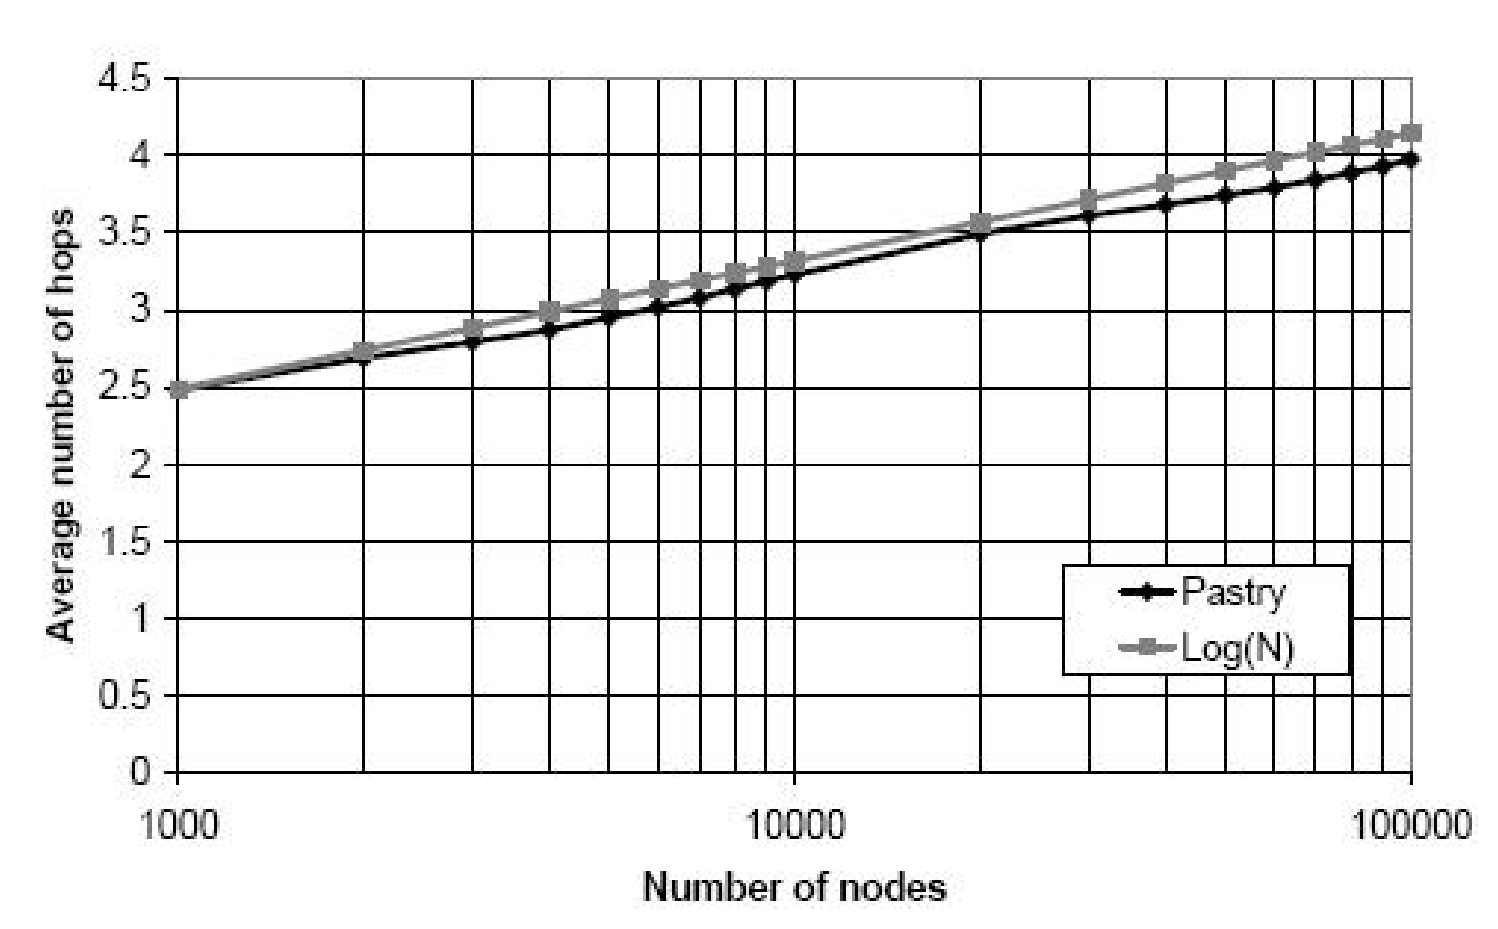
\includegraphics[width=0.8\textwidth]{../images/performance}
  \caption[Pastry und Tapestry: Performance]Routing-Performance bei Pastry und Tapestry \cite{Pastry-Middleware}
  \label{fig:performance}
\end{figure}
Die im Rahmen dieser Ausarbeitung vorgestellten Algorithmen ermöglichen die
Lokalisierung eines Objekts in logarithmischer Zeit zur Anzahl der Knoten
innerhalb eines Netzwerks.


\chapter{Fazit}
Abschlie�end k�nnen wir feststellen, dass die \acr{xml}-Unterst�tzung der untersuchten \acr{dbms} sehr umfangreich ist und viele M�glichkeiten f�r die Verarbeitung von \acr{xml}-Daten bietet. Die f�r das Anwendungsbeispiel aufgestellten Anforderungen konnten mit allen drei \acr{dbms} umgesetzt werden.

Auf der anderen Seite ist die breite Unterst�tzung von \acr{xml}-Funktionalit�ten auch ein Nachteil, da sich der Einarbeitungsaufwand dadurch erh�ht. Bei den "`\acr{xml}-enabled"' Datenbanken steigert sich die Komplexit�t der Anfragen durch Benutzung der \acr{xml}-Funktionen erwartungsgem��.

Die Umsetzung des \acr{sql}/\acr{xml}-Standards ist sowohl bei Oracle 9i wie auch beim SQL-Server 2005 nicht vollst�ndig, wobei Oracle sich wesentlich n�her am Standard orientiert. XPath und XQuery sind beim SQL-Server und eXist vollst�ndiger umgesetzt als bei Oracle. 

Unserer Ansicht nach war der gr��te Nachteil bei der Umsetzung der Anwendung, dass bisher keine Modellierungssprache bei der Verwendung von \acr{xml} existiert. Folglich wird ein strukturiertes Vorgehen bei der Analyse deutlich erschwert. Dieses Problem tritt besonders bei der hybriden Speicherung von \acr{xml}-Daten auf. Wir haben das Problem dadurch umgangen, indem wir uns am bestehenden relationalen Datenmodell orientiert haben.

In unserem Fallbeispiel wurden durch die Benutzung von \acr{xml} keine M�glichkeiten geschaffen, die nicht auch durch die Benutzung von rein relationalen Daten bestanden h�tten. Vorteile h�tten sich ergeben, wenn ein Datenaustausch zwischen den \acr{dbms} existiert h�tte. Beispielsweise wenn die Wohnungsdaten bereits in \acr{xml} vorgelegen h�tten oder ein \acr{xml}-Export der Rechnungsdaten n�tig gewesen w�ren.


%%%
%%% Anhaenge: Glossar, Bibliographie...
%%%

%\cleardoublepage % oder \clearpage
%\phantomsection 

%\appendix
%\pdfbookmark[-1]{\appendixname}{\appendixname} 

%%% Bibliographie-Stil
% abbrvdin, alphadin, plaindin, unsrtdin
\bibliographystyle{alphadin}

%%% Anstatt 'Literatur' -> 'Quellen'
\renewcommand{\bibname}{Quellen}

%%% Bibliographie ausgeben
\bibliography{../Literatur}

%%% Glossar ausgeben
%\printgloss{Glossar}

\end{document}